
\section{Overview}\label{sect:Overview}

This tutorial demonstrates how to specify the models used in a Bayesian ``total-evidence'' phylogenetic analysis of extant and fossil species, combining morphological and molecular data as well as stratigraphic range data from the fossil record \citep[\EG][]{Ronquist2012a,Zhang2016,Gavryushkina2016}.
We begin with a concise introduction to the models used in this analysis in section \ref{sect:Introduction}, followed by a detailed example analysis in section \ref{sect:Exercise} demonstrating how to apply these models in \RevBayes \citep{Hoehna2017a} and use Markov chain Monte Carlo (MCMC) to estimate the posterior distribution of dated phylogenies for data collected from living and fossil bears (family Ursidae).

\bigskip
\subsection{Requirements}\label{subsect:Overview-Requirements}

\subsubsection{Required Software}\label{subsub:Req-Software}
This tutorial requires that you download and install the latest release of \RevBayes \citep{Hoehna2017a}, which is available for Mac OS X, Windows, and Linux operating systems. 
Directions for downloading and installing the software are available on the program webpage:
%\begin{center}
\href{http://revbayes.com/}{http://revbayes.com}.
%\end{center} 

The exercise provided also requires additional programs for editing text files and visualizing output. 
The following are very useful tools for working with \RevBayes:
\begin{itemize}[noitemsep,topsep=0pt]
\item A good text editor -- if you do not already have one that you like, we recommend one that has features for syntax coloring, easy navigation between different files, line numbers, etc.
A good option is \href{http://www.sublimetext.com/}{\tt Sublime Text}, which is available for Mac OSX, Windows, and Linux.
\item \href{http://tree.bio.ed.ac.uk/software/tracer/}{\tt Tracer} -- for visualizing and assessing numerical parameter samples from \RevBayes
\item \href{http://tgvaughan.github.io/icytree/}{\tt IcyTree} -- a web-hosted phylogenetic tree visualization tool that is supported for \href{https://www.mozilla.org/en-US/firefox/products/}{\tt Firefox} or \href{https://www.google.com/chrome/}{\tt Google Chrome} browsers 
\item \href{http://tree.bio.ed.ac.uk/software/figtree/}{\tt FigTree} -- a tree visualization program
\end{itemize}

\subsubsection{Prerequisite Tutorials}
In addition to installing the software, this tutorial assumes that you have read and completed the following tutorials:
\begin{itemize}[noitemsep,topsep=0pt]
\item \href{https://github.com/revbayes/revbayes_tutorial/blob/master/tutorial_TeX/RB_Basics_Tutorial/RB_Basics_Tutorial.pdf}{\mi{Basic Introduction to \Rev and MCMC}}
\item \href{https://github.com/revbayes/revbayes_tutorial/blob/master/tutorial_TeX/RB_MCMC_Intro_Tutorial/RB_MCMC_Intro_Tutorial.pdf}{\mi{Introduction to MCMC Simulation}}
\item \href{https://github.com/revbayes/revbayes_tutorial/blob/master/tutorial_TeX/RB_CTMC_Tutorial/RB_CTMC_Tutorial.pdf}{\mi{Substitution Models}}
\item \href{https://github.com/revbayes/revbayes_tutorial/blob/master/tutorial_TeX/RB_Partition_Tutorial/RB_Partition_Tutorial.pdf}{\mi{Partitioned Data Analysis}}
\end{itemize}


\bigskip
\section{Introduction}\label{sect:Introduction}

The ``total-evidence'' analysis described in this tutorial uses a probabilistic graphical model \citep{Hoehna2014b} integrating three separate likelihood components or data partitions (Fig.\ \ref{fig:module-gm}): one for molecular data (section \ref{subsect:Intro-GTR}), one for morphological data (section \ref{subsect:Intro-Morpho}), and one for fossil stratigraphic range data (section \ref{subsect:Intro-TipSampling}). In addition, all likelihood components are conditioned on a tree topology with divergence times, which is modeled according to a separate prior component (section \ref{subsect:Intro-FBD}).
\begin{figure}[h!]
\fbox{%
\begin{minipage}{\textwidth}\centering
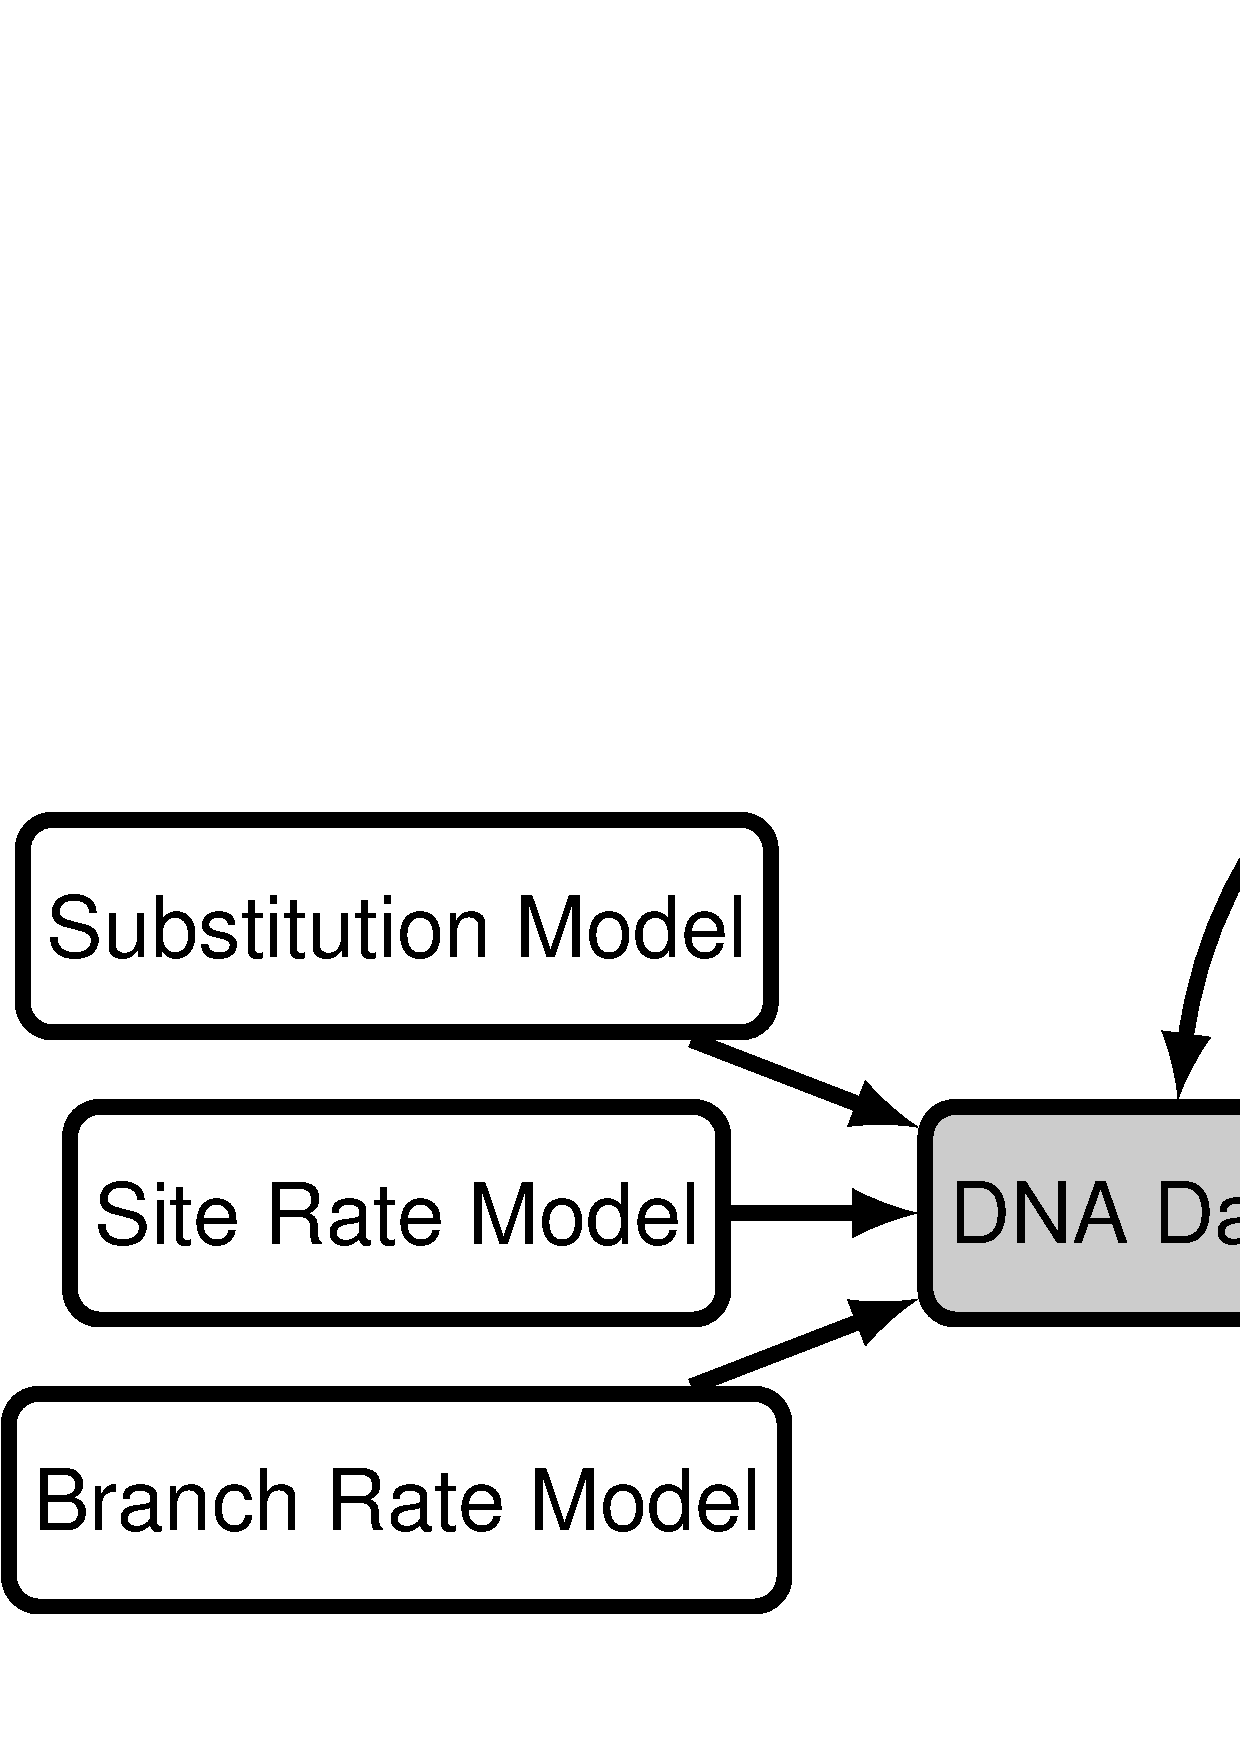
\includegraphics[width=0.92\textwidth,angle=0]{\ResourcePath figures/tikz/full_model_modular}
\caption{\small Modular components of the graphical model used in the ``total-evidence'' analysis described in this tutorial.}
\end{minipage}}
\label{fig:module-gm}
\end{figure}

In figure \ref{fig:example-tree} we provide an example of the type of tree estimated from a total-evidence analysis.
This example shows the complete tree (Fig.\ \ref{fig:example-tree}A) and the sampled or reconstructed tree (Fig.\ \ref{fig:example-tree}B). 
Importantly, we are interested in estimating the topology, divergence times, and fossil sample times of the \textit{reconstructed tree} (Fig.\ \ref{fig:example-tree}B). 
We will describe the distinction between these two trees in section \ref{subsect:Intro-FBD}.
\begin{figure}[h!]
\fbox{%
\begin{minipage}{\textwidth}\centering
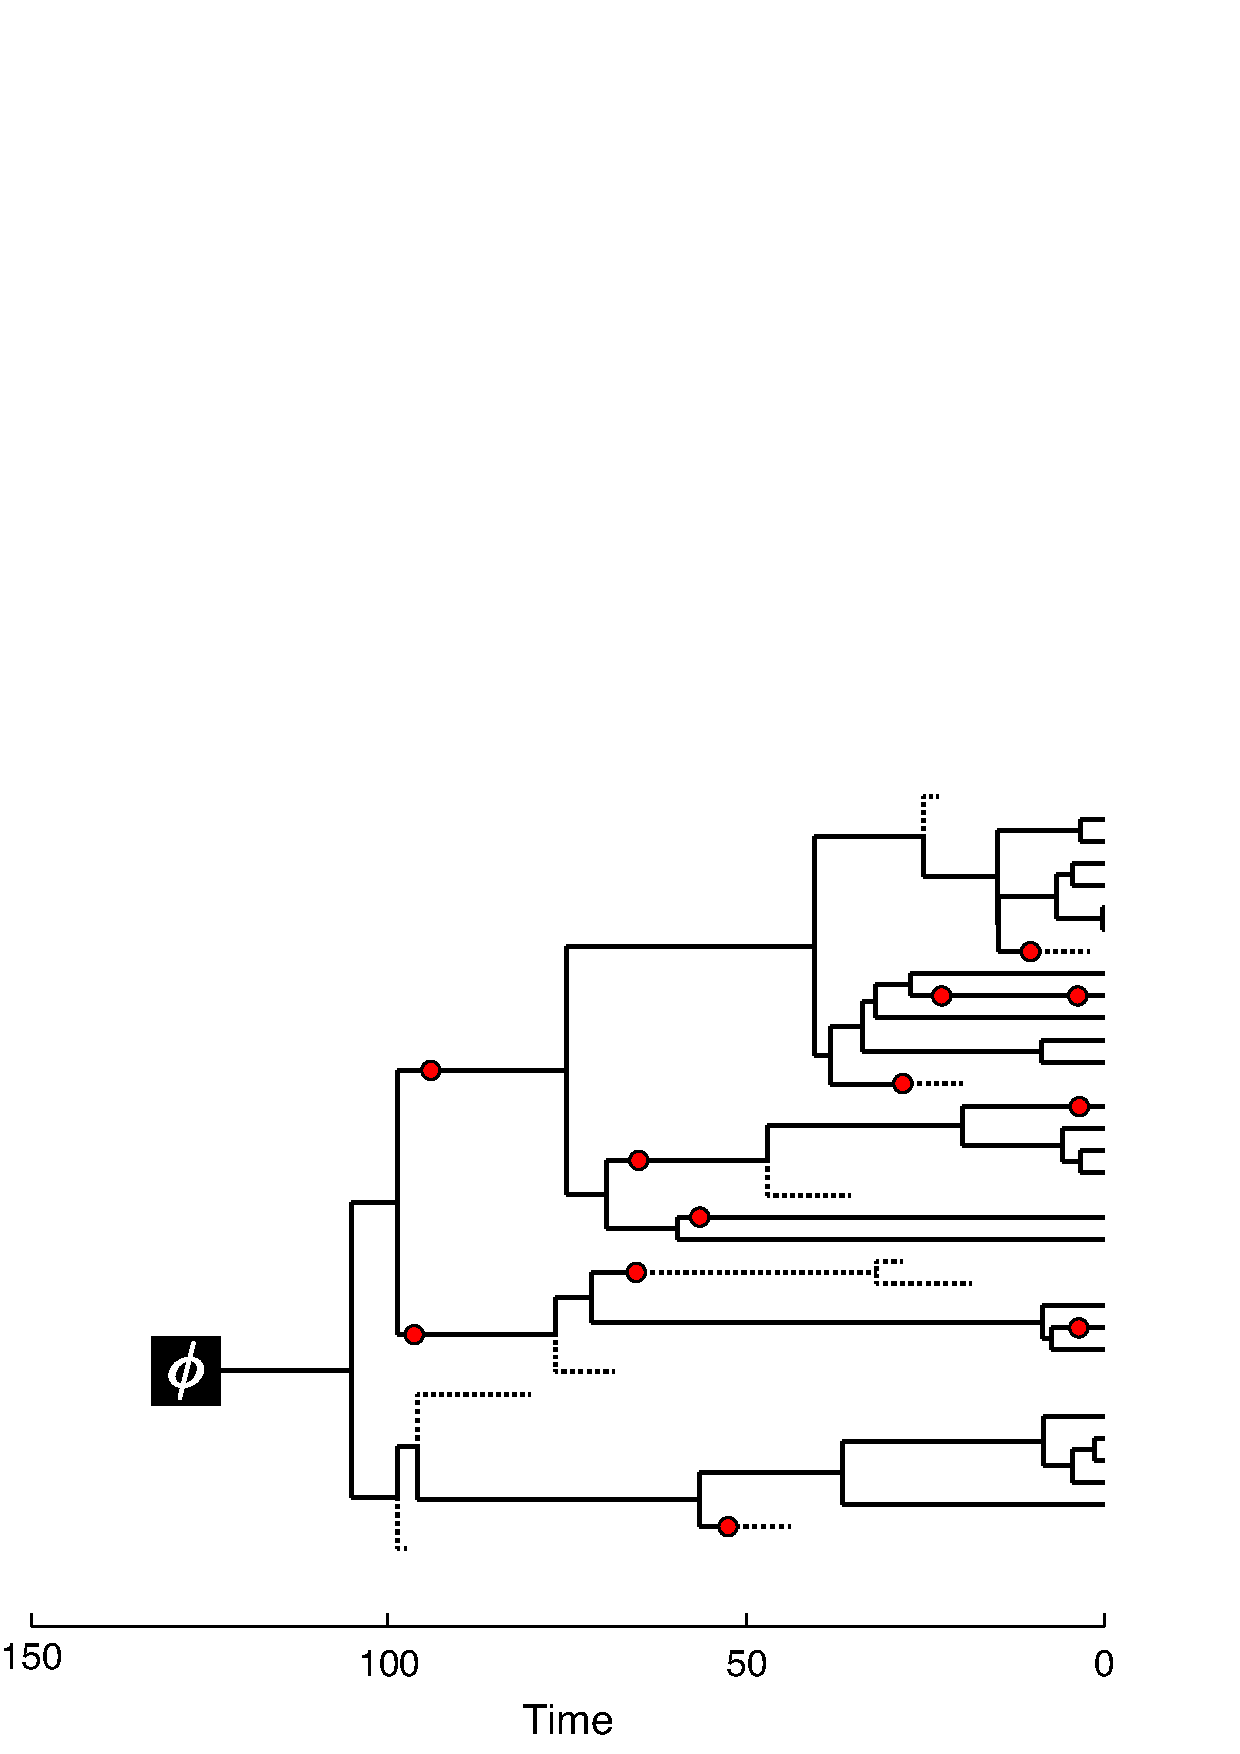
\includegraphics[width=0.44\textwidth,angle=0]{\ResourcePath figures/tree_plot_with_fossils}\hspace{6mm}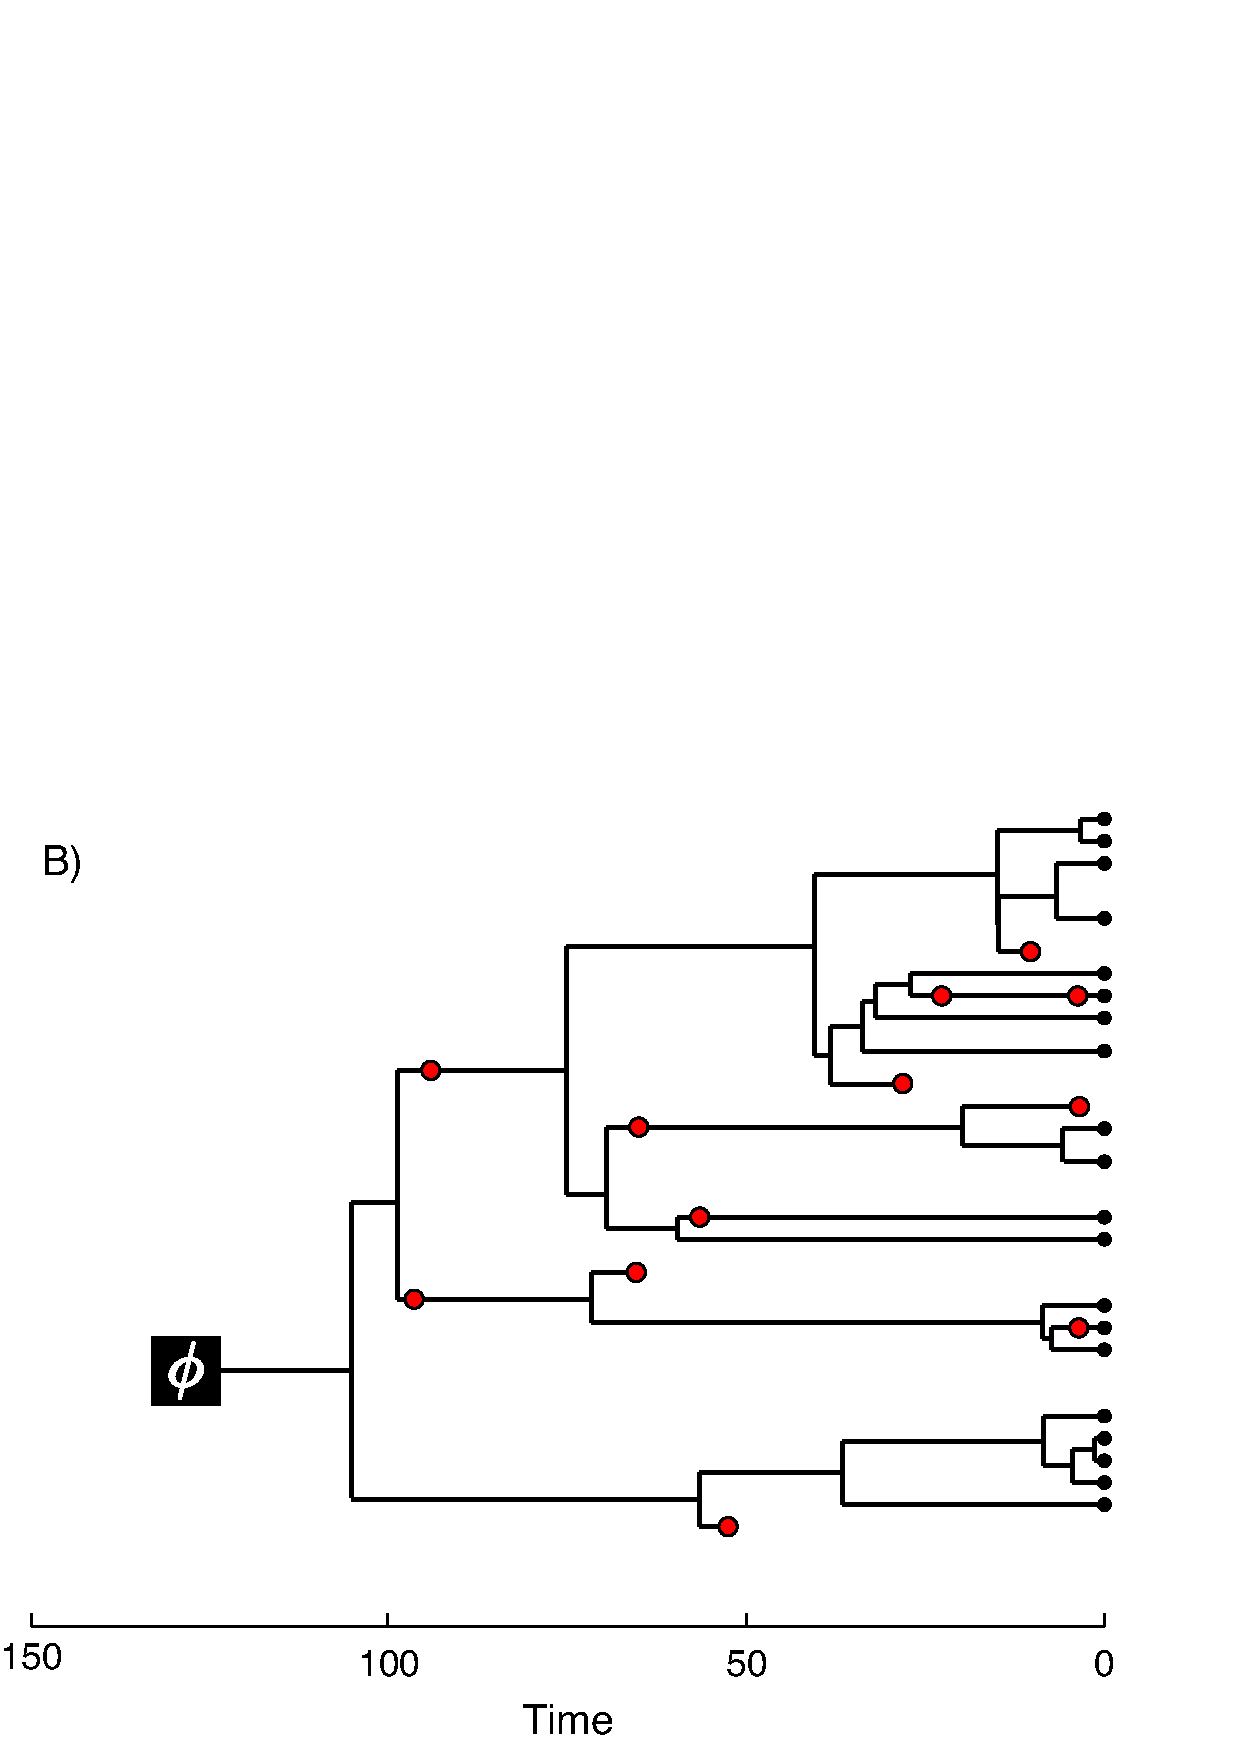
\includegraphics[width=0.44\textwidth,angle=0]{\ResourcePath figures/tree_plot_with_fossils_reconstructed}
\caption{\small One possible realization of the fossilized birth-death (described in section \ref{subsect:Intro-FBD}) process starting at origin time $\phi$, showing fossil sampling events (red circles), and 15 sampled extant taxa (black circles). (A) The complete tree shows all lineages both sampled (solid lines) and unsampled (dotted lines). (B) The reconstructed tree (also called the sampled tree) shows only the sampled lineages.}
\end{minipage}}
\label{fig:example-tree}
\end{figure}


\subsection{Lineage Diversification and Sampling}\label{subsect:Intro-FBD}

The joint prior distribution on tree topologies and divergence times of living and extinct species used in this tutorial is described by the \textit{fossilized birth-death} (FBD) process \citep{Stadler2010, Heath2014}. 
This model simply treats the fossil observations as part of the process governing the tree topology and branch times (the \textsf{Time Tree Model} node in Fig.\ \ref{fig:module-gm}). 
The fossilized birth-death process provides a model for the distribution of speciation times, tree topology, and lineage samples before the present (\EG non-contemporaneous samples like fossils or viruses). 
This type of tree is shown in figure \ref{fig:example-tree}. 
Importantly, this model can be used \textit{with or without} character data for the historical samples. 
Thus, it provides a reasonable prior distribution for analyses combining morphological or DNA data for both extant and fossil taxa---\IE the so-called ``total-evidence'' approaches described by \citet{Ronquist2012a} and extended by \citet{Zhang2016} and \citet{Gavryushkina2016}. 
When matrices of discrete morphological characters for both living and fossil species are unavailable, the fossilized birth-death model imposes a time structure on the tree by \href{https://en.wikipedia.org/wiki/Marginal_distribution}{\textit{marginalizing}} over all possible attachment points for the fossils on the extant tree \citep{Heath2014}, therefore, some prior knowledge of phylogenetic relationships is important.


The FBD model (Fig.\ \ref{fig:fbd_gm}) describes the probability of the tree and fossils conditional on the birth-death parameters: $f[\mathcal{T} \mid \lambda, \mu, \rho, \psi, \phi]$, where $\mathcal{T}$ denotes the tree topology, divergence times, fossil occurrence times, and the times at which the fossils attach to the tree.
%The parameters of the model are:
%\begin{center}
%\begin{tabular}{l c r}
%\hline
%$\lambda$ & & speciation rate\\
%$\mu$ & & extinction rate\\
%$\rho$ & & probability of sampling extant species\\
%$\psi$ & & fossil recovery rate\\
%$\phi$ & & origin time\\
%\hline
%\end{tabular}
%\end{center}
The birth-death parameters $\lambda$ and $\mu$ denote the speciation and extinction rates, respectively. The ``fossilization rate'' or ``fossil recovery rate'' is denoted $\psi$ and describes the rate at which fossils are sampled along lineages of the complete tree. The sampling probability parameter $\rho$ represents the \textit{probability} that an extant species is sampled, and $\phi$ represents the time at which the process originated.

\begin{figure}[h!]
\fbox{%
\begin{minipage}{\textwidth}\centering
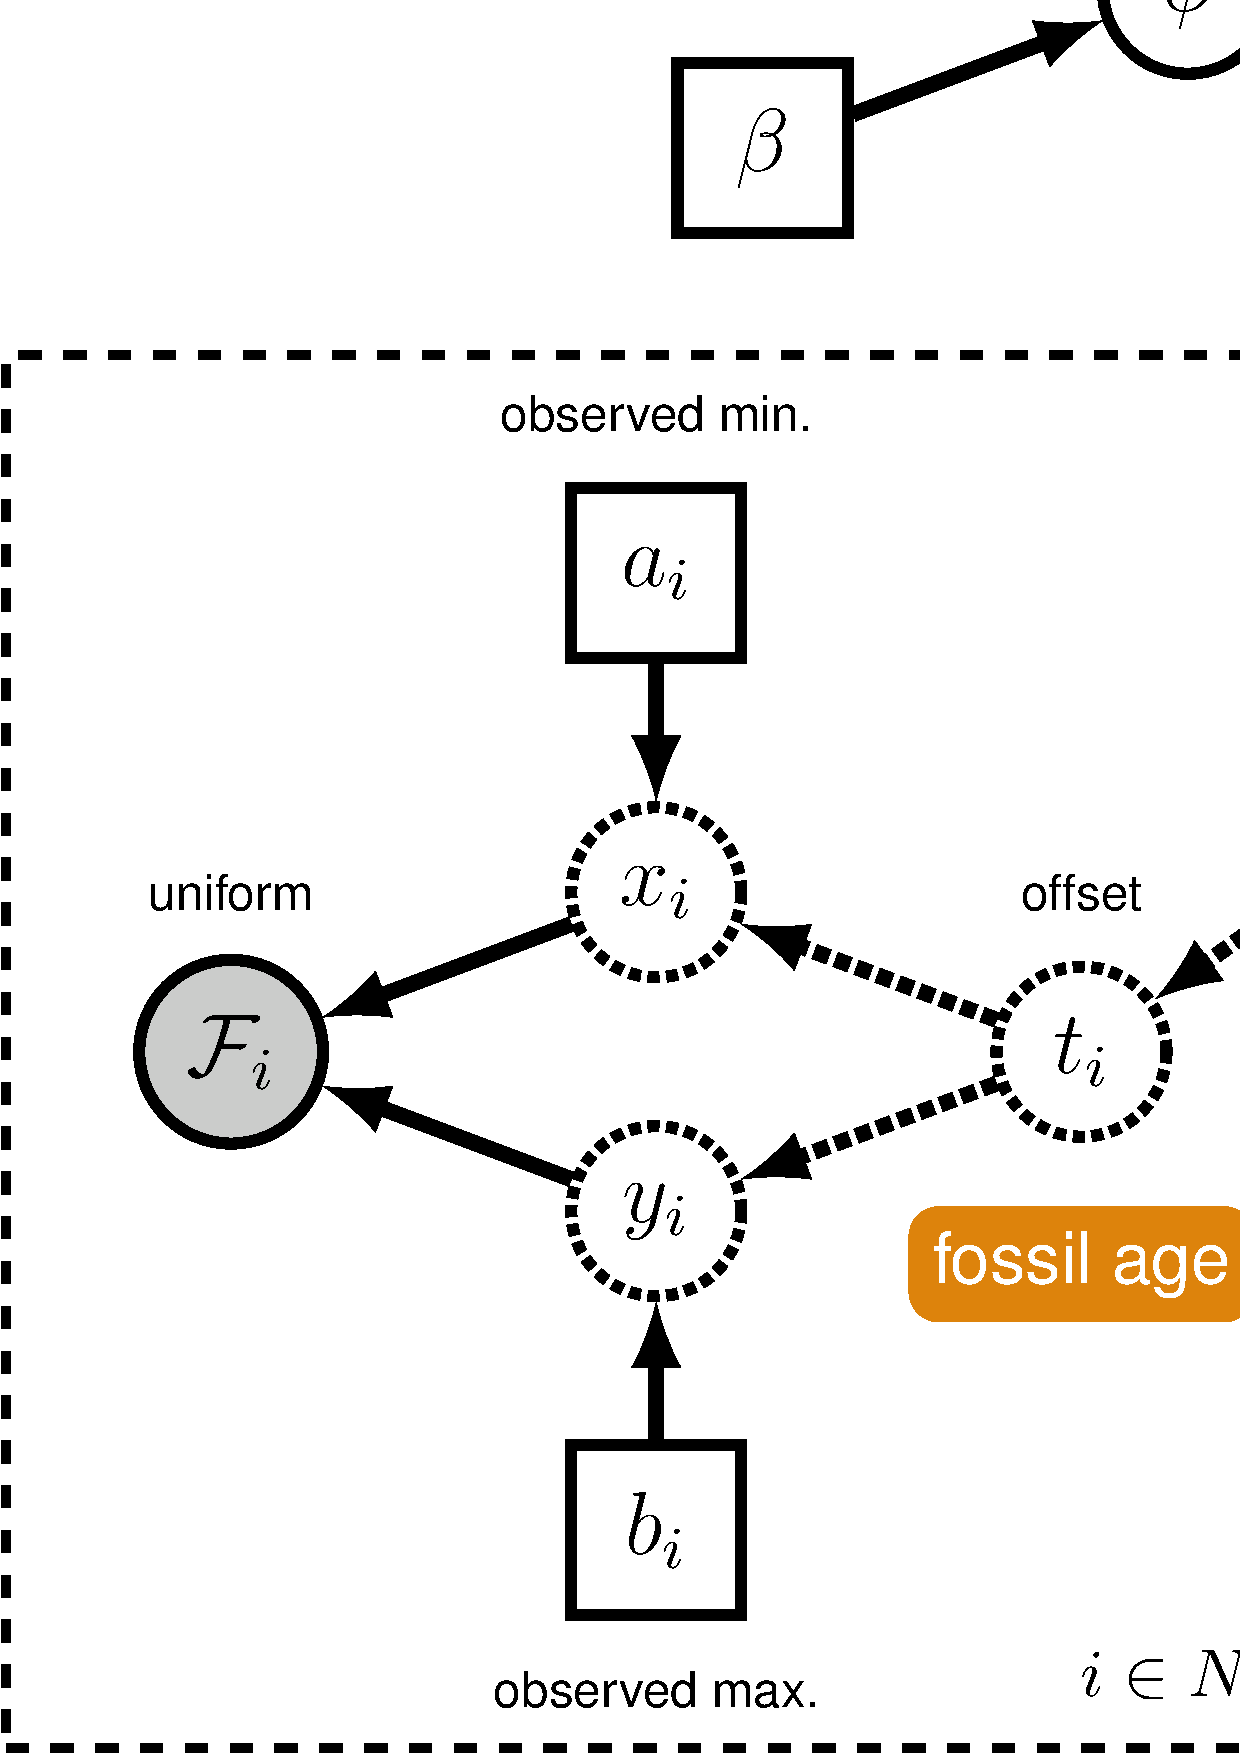
\includegraphics[width=0.58\textwidth,angle=0]{\ResourcePath figures/tikz/fbd_gm}
\caption{\small A graphical model of the fossilized birth-death model describing the generation of the time tree (\textsf{Time Tree Model} in Fig.\ \ref{fig:module-gm}) used in this tutorial. The parameters of the fossilized birth-death process are labeled in orange. The speciation, extinction and fossilization rates are stochastic nodes (circles) drawn from exponential distributions, while the origin time is uniformly distributed. The sampling probability is constant node (square) and equal to one. 
The \textsf{phyloCTMC} represents the phylogenetic continuous-time Markov chain that links the tree model to the other model components and the observed sequence data.
For more information on probabilistic graphical models and their notation, please see \citet{Hoehna2014b}.} 
\end{minipage}}
\label{fig:fbd_gm}
\end{figure}

In the example FBD tree shown in figure \ref{fig:example-tree}, the diversification process originates at time $\phi$, giving rise to $n=20$ species in the present, with both sampled fossils (red circles) and extant species (black circles). 
All of the lineages represented in figure \ref{fig:example-tree}A (both solid and dotted lines) show the \textit{complete tree}. 
This is the tree of all extant \textit{and} extinct lineages generated by the process.
The complete tree is distinct from the \textit{reconstructed tree} (Fig.\ \ref{fig:example-tree}B) which is the tree representing only the lineages sampled as extant taxa or fossils.
Fossil observations (red circles in figure \ref{fig:example-tree}) are recovered over the lifetime of the process along the lineages of the complete tree. 
If a lineage does not have any descendants sampled in the present, it is lost and cannot be observed, these are the dotted lines in figure \ref{fig:example-tree}A. 
The probability must be conditioned on the origin time of the process $\phi$. 
%This can be one of two different nodes in the tree, either the origin time $x_0$ or the root age $x_1$ (Figure \ref{fig:example-tree}).
The origin ($\phi$) of a birth-death process is the starting time of the \textit{stem} lineage, thus this conditions on a single lineage giving rise to the tree.
%Alternatively, a birth-death process can be conditioned on the age of the root ($x_1$), which is the time of the most-recent-common ancestor (MRCA) of the sampled lineages.
%Here, the model assumes that the branching process starts with two lineages, each of which has the same starting time.


An important characteristic of the FBD model is that it accounts for the probability of sampled ancestor-descendant pairs \citep{foote1996}. 
Given that fossils are sampled from lineages in the diversification process, the probability of sampling fossils that are ancestors to taxa sampled at a later date is correlated with the turnover rate ($r=\mu/\lambda$) and the fossil recovery rate ($\psi$).
This feature is important, particularly for datasets with many sampled fossils. 
In the example (Fig.\ \ref{fig:example-tree}), several of the fossils have sampled descendants. These fossils have solid black lines leading to the present. 
%TODO more intro on this section, maybe

\bigskip
\subsection{Incorporating Fossil Stratigraphic Range Data}\label{subsect:Intro-TipSampling}

In order to account for uncertainty in the ages of our fossil species, we can incorporate stratigraphic range information from the fossil record.
We do this by assuming each fossil can occur with uniform probability anywhere within its observed stratigraphic range.
This is somewhat different from the typical approach to node calibration.
Here, instead of treating the calibration density as an additional prior distribution on the tree, we treat it as the \textit{likelihood} of our fossil data given the tree parameter.
Specifically, we assume the likelihood of a particular fossil observation $\mathcal{F}_i$ is equal to one if the fossil's inferred age on the tree $t_i$ falls within its observed stratigraphic range $(a_i,b_i)$, and zero otherwise:
$$f[\mathcal{F}_i \mid a_i, b_i, t_i] = \begin{cases}
1 & \text{if } a_i < t_i < b_i\\
0 & \text{otherwise}
\end{cases}$$
In other words, we assume the likelihood is equal to one if the inferred age is consistent with the fossil record.
We can represent this likelihood in \RevBayes using any uniform distribution that is proportional to the likelihood, \IE non-zero when the likelihood is equal to one (Fig. \ref{fig:tipsampling_gm}).
This model component represents the observed \textsf{Fossil Occurrence Time Data} in the modular graphical model shown in figure \ref{fig:module-gm}.
\begin{figure}[h!]
\fbox{%
\begin{minipage}{\textwidth}\centering
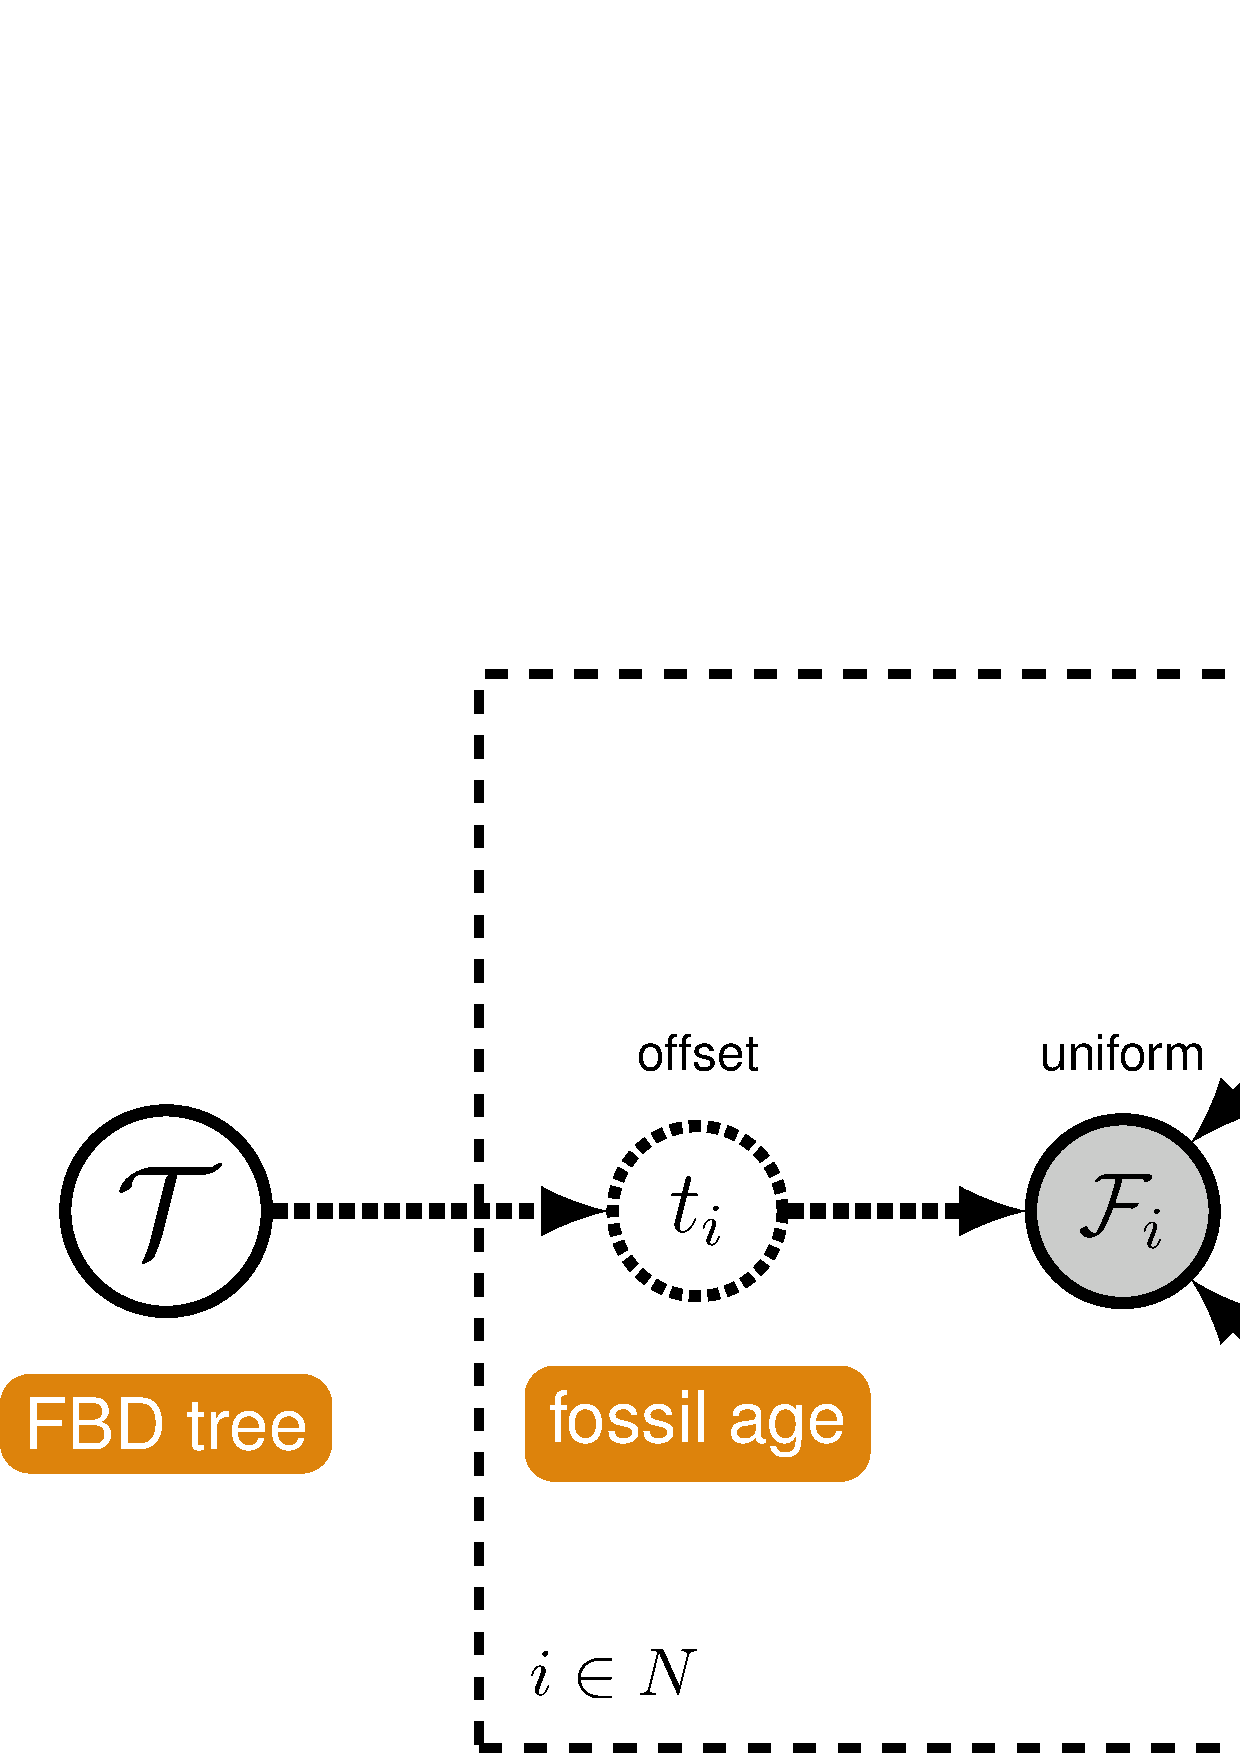
\includegraphics[scale=0.25,angle=0]{\ResourcePath figures/tikz/tipsampling_gm}
\caption{\small A graphical model of the fossil age likelihood model used in this tutorial. The likelihood of fossil observation $\mathcal{F}_i$ is uniform and non-zero when the inferred fossil age $t_i$ falls within the observed stratigraphic range $(a_i,b_i)$.}
\end{minipage}}
\label{fig:tipsampling_gm}
\end{figure}


\subsection{Nucleotide Sequence Evolution}\label{subsect:Intro-GTR}

The model component for the molecular data uses a general time-reversible model of nucleotide evolution and gamma-distributed rate heterogeneity across sites (the \textsf{Substitution Model} and \textsf{Sites Model} in Fig.\ \ref{fig:module-gm}). %TODO cite GTR+G
This model of sequence evolution is covered thoroughly in the \href{https://github.com/revbayes/revbayes_tutorial/raw/master/tutorial_TeX/RB_CTMC_Tutorial/RB_CTMC_Tutorial.pdf}{\mi{Substitution Models}} tutorial.


\subsubsection{Lineage-Specific Rates of Sequence Evolution}\label{subsub:Intro-GTR-UExp}

Rates of nucleotide sequence evolution can vary widely among lineages, and so models that account for this variation by relaxing the assumption of a strict molecular clock \citep{Zuckerkandl1962} can allow for more accurate estimates of substitution rates and divergence times \citep{Drummond2006}.
The simplest type of relaxed clock model assumes that lineage-specific substitution rates are independent or ``uncorrelated''.
One example of such an uncorrelated relaxed model is the uncorrelated \textit{exponential} relaxed clock, in which the substitution rate for each lineage is assumed to be independent and identically distributed according to an exponential density (Fig. \ref{fig:uexp_gm}).
This is the \textsf{Branch Rates Model} for the \textsf{Molecular Data} (\IE Fig.\ \ref{fig:module-gm}) that we will use in this tutorial.
Another possible uncorrelated relaxed clock model is the uncorrelated lognormal model, described in the \href{https://github.com/revbayes/revbayes_tutorial/raw/master/tutorial_TeX/RB_Dating_Tutorial/RB_Dating_Tutorial.pdf}{\mi{Relaxed Clocks}} tutorial \citep[also see][]{Thorne2002,Heath2013}.
\begin{figure}[h!]
\fbox{%
\begin{minipage}{\textwidth}\centering
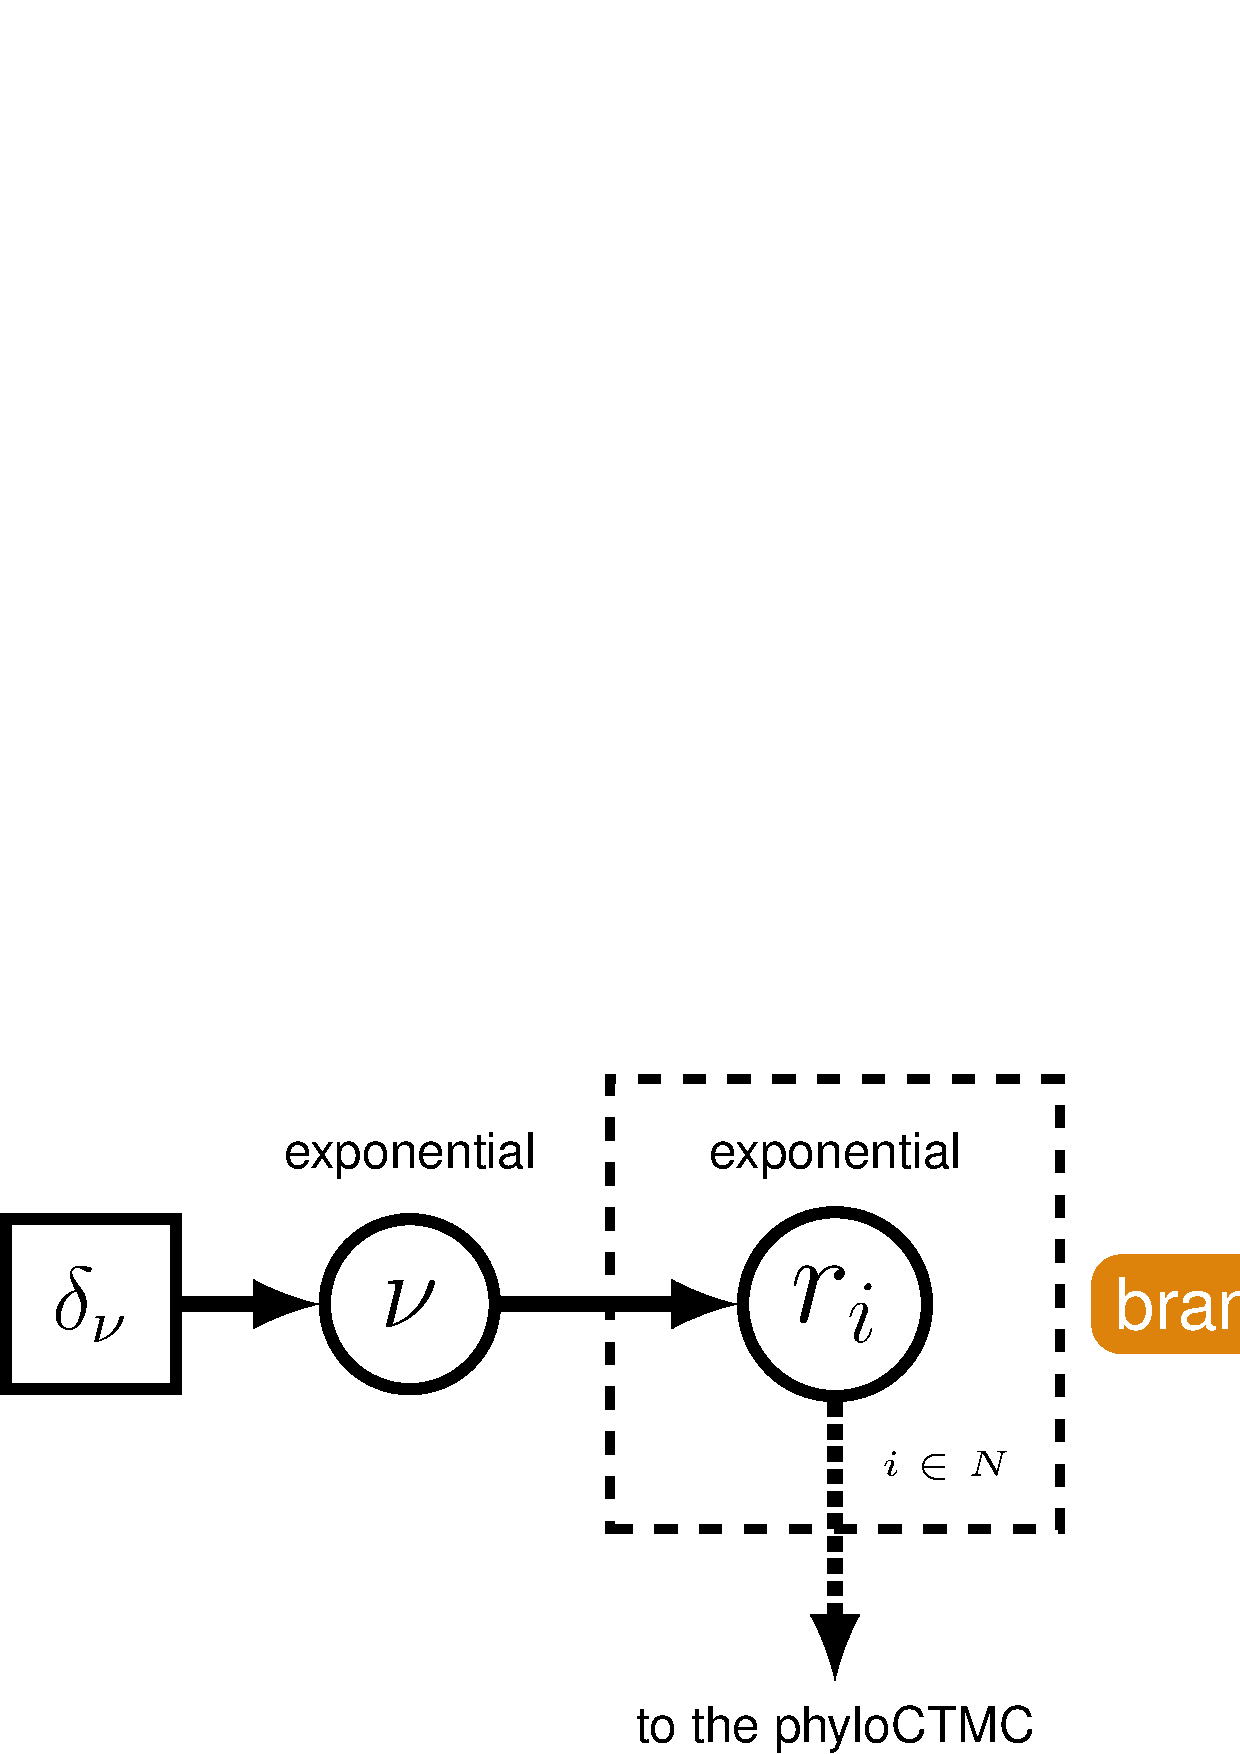
\includegraphics[scale=0.25,angle=0]{\ResourcePath figures/tikz/uexp_gm}
\caption{\small A graphical model of the uncorrelated exponential relaxed clock model. In this model, the clock rate on each branch is independent and identically distributed according to an exponential density with mean drawn from an exponential hyperprior distribution. }
\end{minipage}}
\label{fig:uexp_gm}
\end{figure}


\subsection{Morphological Character Evolution}\label{subsect:Intro-Morpho}

For the vast majority of extinct species, fossil morphology is the primary source of phylogenetically informative characters.
Therefore, an appropriate model of morphological character evolution is needed to reliably infer the positions of these species in a phylogenetic analysis.
The Mk model \citep{Lewis2001} uses a generalized Jukes-Cantor matrix to allow for the incorporation of morphology into likelihood and Bayesian analyses.
One key assumption of this model is that characters exhibit symmetrical change - that a given character is as likely to transition from a one state to another as it is to reverse.
In this tutorial we will consider only binary morphological characters, \IE characters that are coded as being in one of two states, 0 or 1.
For example, the assumption of the Mk model applied to our binary character would mean that a change from a 0 state to a 1 state is as likely as a change from a 1 state to a 0 state.
This assumption is equivalent to assuming that the stationary probability of being in a 1 state is equal to $1/2$.

In this tutorial, we will use Mk to model our data. If you are interested in how we can relax the assumptions in the previous paragraph, please see \href{https://github.com/revbayes/revbayes_tutorial/raw/master/tutorial_TeX/RB_Discrete_Morphology_Tutorial/RB_Discrete_Morphology.pdf}{Discrete Morphology tutorial}.


Because of the way morphological data are collected, we need to exercise caution in how we model the data. 
Traditionally, phylogenetic trees were built from morphological data using parsimony. 
Therefore, only parsimony informative characters were collected---that is, characters that are useful for discriminating between phylogenetic hypotheses under the maximum parsimony criterion.
This means that many morphological datasets do not contain invariant characters or \href{https://en.wikipedia.org/wiki/Autapomorphy}{autapomorphies}, as these are not parsimony informative. 
However, by excluding these slow-evolving characters, estimates of the branch lengths can be inflated \citep{Felsenstein1992,Lewis2001}.
Therefore, it is important to use models that can condition on this data-acquisition bias. 
\RevBayes has two ways of doing this: one is used for datasets in which only parsimony informative characters are observed; the other is for datasets in which parsimony informative characters and parsimony uninformative variable characters (such as autapomorphies) are observed.


\subsubsection{The Morphological Clock}\label{subsub:Intro-MorphClock}

%TODO write about the morphological clock


Just like with the molecular data (section \ref{subsub:Intro-GTR-UExp}), our observations of discrete morphological characters are conditional on the rate of change along each branch in the tree. 
This model component defines the \textsf{Branch Rate Model} of the \textsf{Morphological Data} in the generalized graphical model shown in figure \ref{fig:module-gm}.
The relaxed clock model we described for the molecular data in section \ref{subsub:Intro-GTR-UExp} it allows the substitution rate to vary through time and among lineages. 
For the morphological data, we will instead use a ``strict clock'' model \citep{Zuckerkandl1962}, in which the rate of discrete character change is assumed to be constant throughout the tree.
The strict clock is the simplest morphological branch rate model we can construct (graphical model shown in Fig.\ \ref{fig:morph_clock_gm}).
\begin{figure}[h!]
\fbox{%
\begin{minipage}{\textwidth}\centering
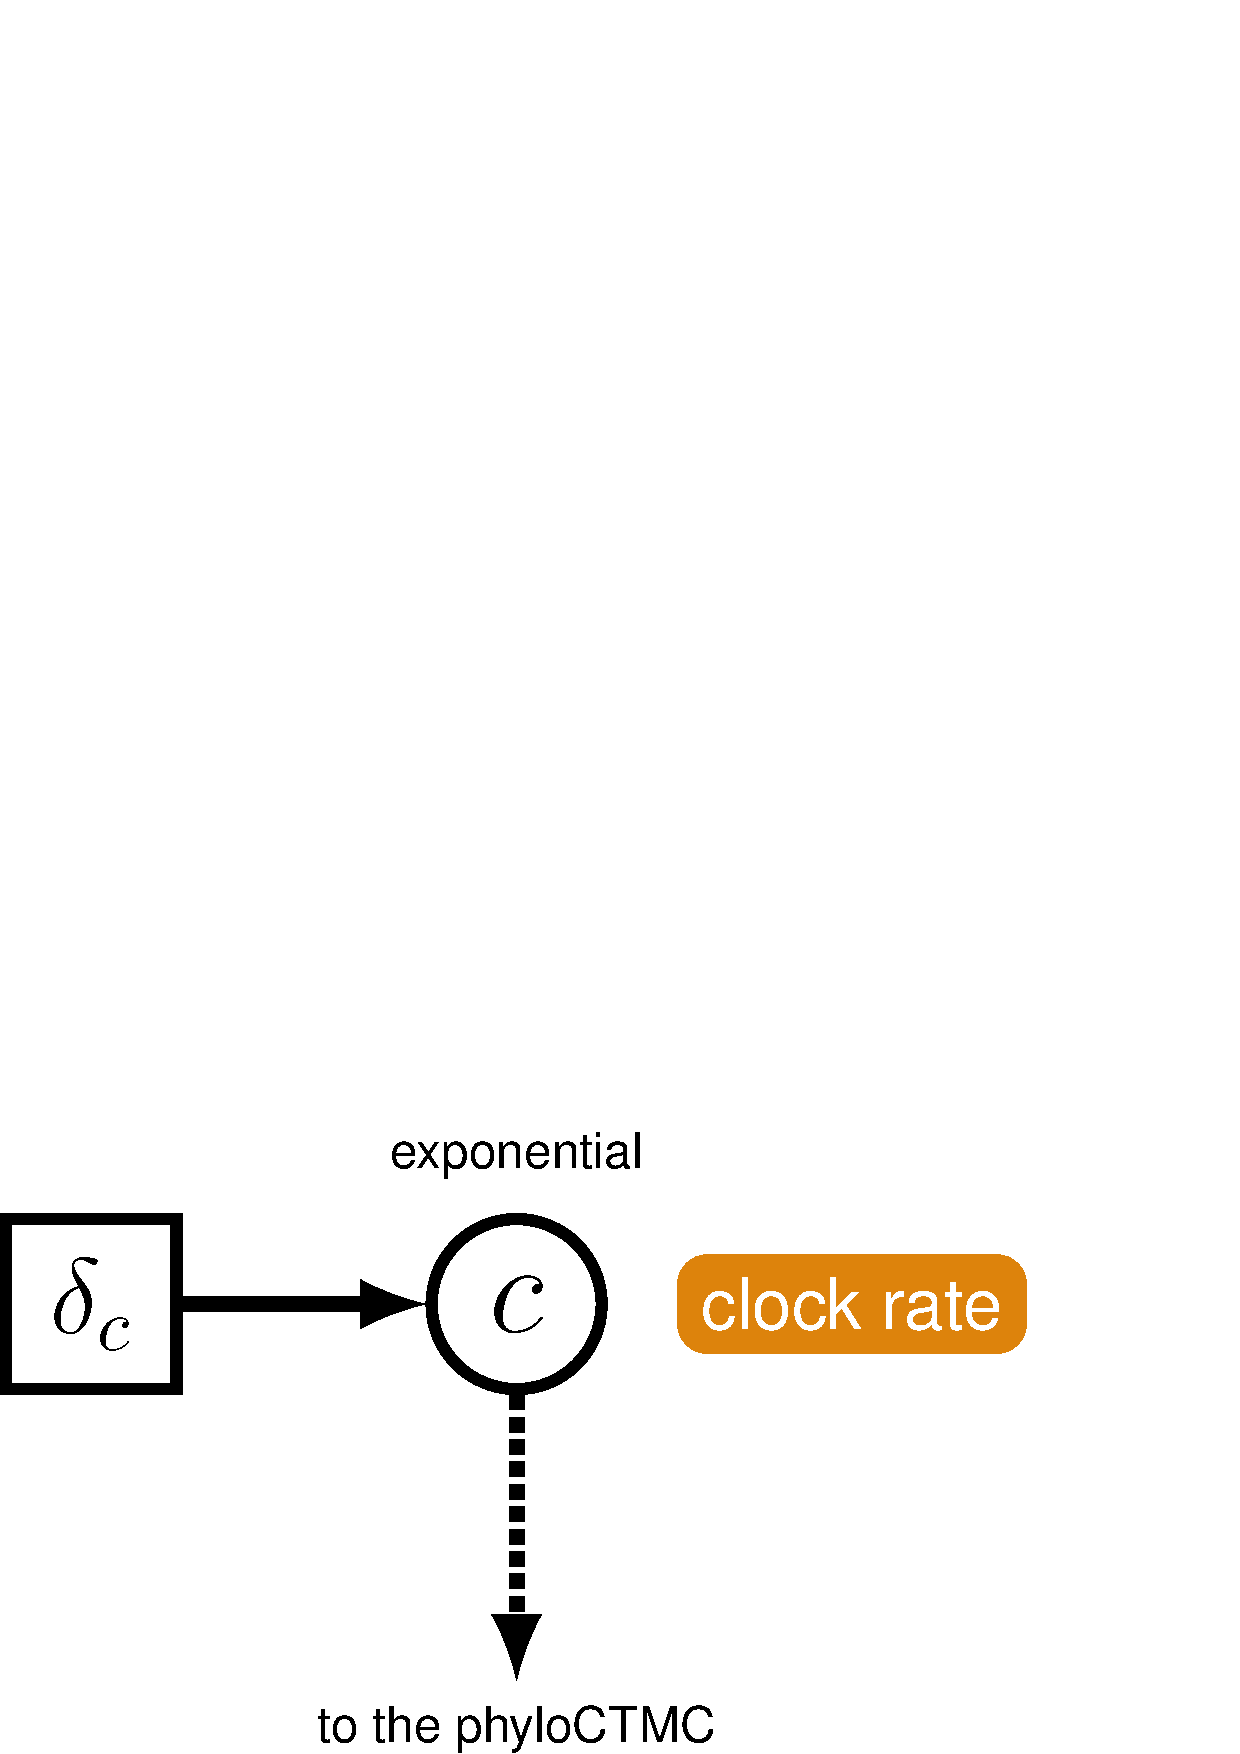
\includegraphics[scale=0.25,angle=0]{\ResourcePath figures/tikz/morph_clock_gm}
\caption{\small The graphical-model representation of the branch-rate model governing the evolution of morphological characters. This model is consistent with a strict morphological clock, where every branch has the same rate of change ($c$) and that rate is drawn from an exponential distribution with a rate parameter of $\delta_c$.}
\end{minipage}}
\label{fig:morph_clock_gm}
\end{figure} 


\bigskip
\section{Example: Estimating the Phylogeny and Divergence Times of Fossil and Extant Bears}\label{sect:Exercise}

In this exercise, we will combine different types of data from 22 species of extant and extinct bears to estimate a posterior distribution of calibrated time trees for this group.
%The analysis in this tutorial includes data from several different sources (see Fig.\ \ref{fig:module-gm}).
We have molecular sequence data for ten species, which represent all of the eight living bears and two extinct species sequenced from sub-fossil specimens (\textit{Arctodus simus, Ursus spelaeus}).
The sequence alignment provided is a 1,000 bp fragment of the cytochrome-b mitochondrial gene \citep{krause2008}.
The morphological character matrix unites 18 taxa (both fossil and extant) with 62 binary (states \cl{0} or \cl{1}) characters \citep{abella12}.
%Further, we must provide an occurrence time for each taxon sampled from the fossil record.
For the fossil species, occurrence times are obtained from the literature or fossil databases like the \href{http://fossilworks.org/}{Fossilworks PaleoDB} or the \href{http://fossilcalibrations.org/}{Fossil Calibration Database}, or from your own paleontological expertise. 
The 14 fossil species used in this analysis are listed in Table \ref{bearFossilTable} along with the age range for the species and relevant citation.
%For this exercise, we will fix the ages to a value within the age range provided in Table \ref{bearFossilTable}. 
Finally, there are two fossil species (\textit{Parictis montanus, Ursus abstrusus}) for which we do not have morphological character data (or molecular data) and we must use prior information about their phylogenetic relationships to incorporate these taxa in our analysis. 
This information will be applied using clade constraints.

\begin{table}[tbh!]
\centering
\caption{Fossil species used for calibrating divergence times under the FBD model. Modified from Table S.3 in the supplemental appendix of \citet{Heath2014}.}\label{bearFossilTable}
{\small
\begin{tabular}{@{\extracolsep{\fill}}l  c c c r}
\hline
\multicolumn{1}{@{}l}{\textbf{Fossil species}}  & &\multicolumn{1}{c}{\textbf{Age range (My)}}  & &\multicolumn{1}{r}{\textbf{Citation}} \\ 
\hline
\hspace{2mm} \textit{Parictis montanus} & & 33.9--37.2 & & \cite{clark1972,krause2008}\\
\hspace{2mm} \textit{Zaragocyon daamsi} & & 20--22.8  & & \cite{ginsburg1995,abella12}\\
\hspace{2mm} \textit{Ballusia elmensis} & & 13.7--16 & & \cite{ginsburg1998,abella12}\\
\hspace{2mm} \textit{Ursavus primaevus} & & 13.65--15.97 & & \cite{andrews1977,abella12}\\
\hspace{2mm} \textit{Ursavus brevihinus} & & 15.97--16.9  & & \cite{heizmann1980,abella12}\\
\hspace{2mm} \textit{Indarctos vireti} & & 7.75--8.7  & & \cite{montoya2001,abella12}\\
\hspace{2mm} \textit{Indarctos arctoides} & & 8.7--9.7 & & \cite{geraads2005,abella12}\\
\hspace{2mm} \textit{Indarctos punjabiensis} & & 4.9--9.7 & & \cite{baryshnikov2002,abella12}\\
\hspace{2mm} \textit{Ailurarctos lufengensis} & & 5.8--8.2 & & \cite{jin2007,abella12}\\
\hspace{2mm} \textit{Agriarctos spp.} & & 4.9--7.75 && \cite{abella2011,abella12}\\
\hspace{2mm} \textit{Kretzoiarctos beatrix} & & 11.2--11.8 & & \cite{abella2011,abella12}\\
\hspace{2mm} \textit{Arctodus simus} & & 0.012--2.588 & & \cite{churcher1993,krause2008}\\
\hspace{2mm} \textit{Ursus abstrusus} & & 1.8--5.3 & & \cite{bjork1970,krause2008}\\
\hspace{2mm} \textit{Ursus spelaeus} & & 0.027--0.25 & & \cite{loreille2001,krause2008}\\
\hline
\end{tabular}}
\end{table}


%The dataset we will use encompasses 8 extant species and 14 fossil species, consisting of morphological data for 18 species, nucleotide sequence data from 10 species, and stratigraphic fossil range data for all 14 fossil species.
%Two fossil species do not have any morphological or molecular data.

\medskip
\subsection{Tutorial Format}\label{subsect:Exercise-Format}

This tutorial follows a specific format for issuing instructions and information.

{\begin{framed}
The boxed instructions guide you to complete tasks that are not part of the \RevBayes syntax, but rather direct you to create directories or files or similar.
\end{framed}}

Information describing the commands and instructions will be written in paragraph-form before or after they are issued.

All command-line text, including all \Rev syntax, are given in \cl{monotype font}. 
Furthermore, blocks of \Rev code that are needed to build the model, specify the analysis, or execute the run are given in separate shaded boxes.
For example, we will instruct you to create a constant node called \cl{rho} that is equal to \cl{1.0} using the \cl{<-} operator like this:
%Load the cytochrome-b sequences from file and assign the data matrix to a variable called \cl{cytb}.
{\tt \begin{snugshade*}
\begin{lstlisting}
rho <- 1.0
\end{lstlisting}
\end{snugshade*}}

It is important to be aware that some PDF viewers may render some characters given as \colorbox{shadecolor}{\tt{Rev commands}} differently. 
Thus, if you copy and paste text from this PDF, you may introduce some incorrect characters. 
Because of this, we recommend that you type the instructions in this tutorial or copy them from the scripts provided. 


\medskip
\subsection{Data and Files}\label{subsect:Exercise-DataFiles}

{\begin{framed}
On your own computer, create a directory called {\textcolor{red}{\cl{RB\_TotalEvidenceDating\_FBD\_Tutorial}}} (or any name you like). 

In this directory download and unzip the archive containing the data files: \href{https://github.com/revbayes/revbayes_tutorial/raw/master/RB_TotalEvidenceDating_FBD_Tutorial/data.zip}{\cl{data.zip}}.

This will create a folder called \cl{data} that contains the files necessary to complete this exercise.
\end{framed}}


%We provide the data files which we will use in this tutorial.
%You may want to use your own data instead.
In the \cl{data} folder, you will find the following files:
\begin{itemize}[noitemsep,topsep=0pt]
\item \cl{bears\_taxa.tsv}: a tab-separated table listing every bear species (both fossil and extant) and their occurrence dates. For extant taxa, the occurrence date is \cl{0.0} (\IE the present) and for fossil species, the occurrence date is equal to the mean of the age range (the ranges are defined in a separate file).
\item \cl{bears\_cytb.nex}: an alignment in NEXUS format of 1,000 bp of cytochrome b sequences for 10 bear species. This alignment includes 8 living bears and 2 extinct sub-fossil bears.
\item \cl{bears\_morphology.nex}: a matrix of 62 discrete, binary (coded \cl{0} or \cl{1}) morphological characters for 18 species of fossil and extant bears.
\item \cl{bears\_fossil\_intervals.tsv}: a tab-separated table containing the age ranges (minimum and maximum in millions of years) for 14 fossil bears.
\end{itemize}

\bigskip
\subsection{Getting Started}\label{subsect:Exercise-GetStart}

{\begin{framed}
Create a new directory (in \cl{RB\_TotalEvidenceDating\_FBD\_Tutorial}) called {\textcolor{red}{\cl{scripts}}}. (If you do not have this folder, please refer to the directions in section \ref{subsect:Exercise-DataFiles}.)
\end{framed}}

When you execute \RevBayes in this exercise, you will do so within the main directory you created (\cl{RB\_TotalEvidenceDating\_FBD\_Tutorial}), thus, if you are using a Unix-based operating system, we recommend that you add the \RevBayes binary to your path.

%TODO Stuff about how to start or Rev basics?

%We will complete this analysis in \RevBayes by entering the \Rev code interactively. 
%
%Note that some PDF viewers render some characters differently and if you copy/paste directly from this document, you may introduce erroneous characters. 
%This can cause commands to fail. 
%For learning, it's often better to `live code' and type the commands in manually, rather than copying and pasting. 
%
%Hints for navigating in the \RevBayes console:
%\begin{itemize}[noitemsep,topsep=0pt]
%    \item \cl{Ctrl+A} -- jump to the beginning of the line
%    \item \cl{Ctrl+E} -- jump to the end of the line
%    \item Pressing the up key will pull up previous commands, and allow you to edit them
%    \item If you enter the first few letters of a \RevBayes keyword and then the \textsc{Tab} key, this will `autocomplete' the remaining letters.
%    \item Help -- if you type \cl{?} followed immediately by a \RevBayes keyword, this will print the help pages for that keyword to the screen. (Example \cl{?dnBDP})
%\end{itemize}
%%In \RevBayes, \cl{Ctrl+A} allows you to jump to the start of the command, if you need to delete extra characters from the front of a line. \cl{Ctrl+E} allows you to jump to the end of a command. Pressing the up key will pull up previous commands, and allow you to edit them. If you do choose to copy and paste in commands, doing that from the tutorial script file will cause fewer errors. 

\bigskip

\subsection{Creating \Rev Files}\label{subsect:Exercise-CreatingFiles}

For complex models and analyses, it is best to create \Rev script files that will contain all of the model parameters, moves, and functions. 
In this exercise, you will work primarily in your text editor\footnote{In section \ref{subsub:Req-Software} we offer a recommendation for a text editor.} and create a set of modular files that will be easily managed and interchanged.
You will write the following files from scratch and save them in the \cl{scripts} directory:
\begin{itemize}[noitemsep,topsep=0pt]
\item \cl{mcmc\_TEFBD.Rev}: the master \Rev file that loads the data, the separate model files, and specifies the monitors and MCMC sampler.
\item \cl{model\_FBDP\_TEFBD.Rev}: specifies the model parameters and moves required for the fossilized birth-death prior on the tree topology, divergence times, fossil occurrence times, and diversification dynamics.
\item \cl{model\_UExp\_TEFBD.Rev}: specifies the components of the uncorrelated exponential model of lineage-specific substitution rate variation.
\item \cl{model\_GTRG\_TEFBD.Rev}: specifies the parameters and moves for the general time-reversible model of sequence evolution with gamma-distributed rates across sites (GTR+$\Gamma$).
\item \cl{model\_Morph\_TEFBD.Rev}: specifies the model describing discrete morphological character change (binary characters) under a strict morphological clock. 
\end{itemize}

All of the files that you will create are also provided in the \RevBayes tutorial repository\footnote{\url{https://github.com/revbayes/revbayes_tutorial/tree/master/RB_TotalEvidenceDating_FBD_Tutorial/scripts}}. 
Please refer to these files to verify or troubleshoot your own scripts. 
%TODO add link to scripts


\bigskip
\subsection{Start the Master \Rev File and Import Data}\label{subsect:Exercise-StartMasterRev}



{\begin{framed}
Open your text editor and create the master \Rev file called {\textcolor{red}{\cl{mcmc\_TEFBD.Rev}}} in the \cl{scripts} directory.

Enter the \Rev code provided in this section in the new model file.
\end{framed}}

The file you will begin in this section will be the one you load into \RevBayes when you've completed all of the components of the analysis.
In this section you will begin the file and write the \Rev commands for loading in the taxon list and managing the data matrices.
Then, starting in section \ref{subsect:Exercise-ModelFBD}, you will move on to writing module files for each of the model components. 
Once the model files are complete, you will return to editing \cl{mcmc\_TEFBD.Rev} and complete the \Rev script with the instructions given in section \ref{subsect:Exercise-CompleteMCMC}.

%{\footnotesize{This file is provided in the \RevBayes tutorial repository: \href{https://github.com/revbayes/revbayes_tutorial/blob/master/RB_TotalEvidenceDating_FBD_Tutorial/scripts/mcmc_TEFBD.Rev}{\cl{mcmc\_TEFBD.Rev}}.}}

\medskip
\subsubsection{Load Taxon List}\label{subsub:Exercise-TaxList}

Begin the \Rev script by loading in the list of taxon names from the \cl{bears\_taxa.tsv} file using the \cl{readTaxonData()} function.
\begin{snugshade*}
\begin{lstlisting}
taxa <- readTaxonData("data/bears_taxa.tsv")
\end{lstlisting}
\end{snugshade*}
This function reads a tab-delimited file and creates a variable called \cl{taxa} that is a list of all of the taxon names relevant to this analysis. 
This list includes all of the fossil and extant bears.



\medskip
\subsubsection{Load Data Matrices}\label{subsub:Exercise-LoadData}

\RevBayes uses the function \cl{readDiscreteCharacterData()} to load a data matrix to the workspace from a formatted file. 
This function can be used for both molecular sequences and discrete morphological characters.

Load the cytochrome-b sequences from file and assign the data matrix to a variable called \cl{cytb}.
{\tt \begin{snugshade*}
\begin{lstlisting}
cytb <- readDiscreteCharacterData("data/bears_cytb.nex") 
\end{lstlisting}
\end{snugshade*}}

Next, import the morphological character matrix and assign it to the variable \cl{morpho}. 
{\tt \begin{snugshade*}
\begin{lstlisting}
morpho <- readDiscreteCharacterData("data/bears_morphology.nex")
\end{lstlisting}
\end{snugshade*}}

 

\medskip
\subsubsection{Add Missing Taxa}\label{subsub:Exercise-AddMissing}

In the descriptions of the files in section \ref{subsect:Exercise-DataFiles}, we mentioned that the two data matrices have different numbers of taxa. 
Thus, we must add any taxa that are not found in the molecular (\cl{cytb}) partition (\IE are only found in the fossil data) to that data matrix as missing data (with \cl{?} in place of all characters), and do the same with the morphological data partition (\cl{morpho}).
In order for all the taxa to appear on the same tree, they all need to be part of the same dataset, as opposed to present in separate datasets. 
This ensures that there is a unified taxon set that contains all of our tips.
{\tt \begin{snugshade*}
\begin{lstlisting}
cytb.addMissingTaxa( taxa )
morpho.addMissingTaxa( taxa )
\end{lstlisting}
\end{snugshade*}}


\medskip
\subsubsection{Create Helper Variables}\label{subsub:Exercise-mviVar}

Before we begin writing the \Rev scripts for each of the model components, we need to instantiate a couple ``helper variables'' that will be used by downstream parts of our model specification files. 
These variables will be used in more than one of the module files so it's best to initialize them in the master file.

Create a new constant node called \cl{n\_taxa} that is equal to the number of species in our analysis (22). 
{\tt \begin{snugshade*}
\begin{lstlisting}
n_taxa <- taxa.size() 
\end{lstlisting}
\end{snugshade*}}

Next, create a workspace variable called \cl{mvi}. 
This variable is an iterator that will build a vector containing all of the MCMC moves used to propose new states for every stochastic node in the model graph. 
Each time a new move is added to the vector, \cl{mvi} will be incremented by a value of \cl{1}.
{\tt \begin{snugshade*}
\begin{lstlisting}
mvi = 1
\end{lstlisting}
\end{snugshade*}}
One important distinction here is that \cl{mvi} is part of the \RevBayes workspace and not the hierarchical model. 
Thus, we use the workspace assignment operator \cl{=} instead of the constant node assignment \cl{<-}. 

{\begin{framed}
Save your current working version of \cl{mcmc\_TEFBD.Rev} in the \cl{scripts} directory.

We will now move on to the next \Rev file and will complete \cl{mcmc\_TEFBD.Rev} in section \ref{subsect:Exercise-CompleteMCMC}.
\end{framed}}


\bigskip
\subsection{The Fossilized Birth-Death Process}\label{subsect:Exercise-ModelFBD}

{\begin{framed}
Open your text editor and create the fossilized birth-death model file called {\textcolor{red}{\cl{model\_FBDP\_TEFBD.Rev}}} in the \cl{scripts} directory.

Enter the \Rev code provided in this section in the new model file.
\end{framed}}

This file will define the models described in sections \ref{subsect:Intro-FBD} and \ref{subsect:Intro-TipSampling} above.
If necessary, please review the graphical models depicted for the fossilized birth-death process (Fig.\ \ref{fig:fbd_gm}) and the likelihood of the tip sampling process (Fig.\ \ref{fig:tipsampling_gm}).

\subsubsection{Speciation and Extinction Rates}\label{subsub:Exercise-FBD-SpeciationExtinction}

Two key parameters of the FBD process are the speciation rate (the rate at which lineages are added to the tree, denoted by $\lambda$ in Fig.\ \ref{fig:fbd_gm}) and the extinction rate (the rate at which lineages are removed from the tree, $\mu$ in Fig.\ \ref{fig:fbd_gm}). 
We'll place exponential priors on both of these values. 
%An exponential prior with a $\lambda$ =  10 places a higher probability on values closer to zero than one for these parameters. 
Each parameter is assumed to be drawn independently from a different exponential distribution with rates $\delta_{\lambda}$ and $\delta_{\mu}$ respectively (see Fig.\ \ref{fig:fbd_gm}). 
Here, we will assume that $\delta_{\lambda} = \delta_{\mu} = 10$. 
Note that an exponential distribution with $\delta = 10$ has an expected value (mean) of $1/10$. 

Create the exponentially distributed stochastic nodes for the \cl{speciation\_rate} and \cl{extinction\_rate} using the \cl{\textasciitilde} operator.
{\tt \begin{snugshade*}
\begin{lstlisting}
speciation_rate ~ dnExponential(10)
extinction_rate ~ dnExponential(10)
\end{lstlisting}
\end{snugshade*}}

For every stochastic node we declare, we must also specify proposal algorithms (called \textit{moves}) to sample the value of the parameter in proportion to its posterior probability.
If a move is not specified for a stochastic node, then it will not be estimated, but fixed to its initial value. 

The rate parameters for extinction and speciation are both real, positive numbers (\IE floating point variables). 
For both of these nodes, we will use a scaling move (\cl{mvScale()}), which proposes multiplicative changes to a parameter.
Many moves also require us to set a \textit{tuning value}, called \cl{lambda} for \cl{mvScale()}, which determine the size of the proposed change. 
Here, we will use three scale moves for each parameter with  different values of lambda. 
By using multiple moves for a single parameter, we will improve the mixing of the Markov chain. 
{\tt \begin{snugshade*}
\begin{lstlisting}
moves[mvi++] = mvScale(speciation_rate, lambda=0.01, weight=1)
moves[mvi++] = mvScale(speciation_rate, lambda=0.1,  weight=1)
moves[mvi++] = mvScale(speciation_rate, lambda=1.0,  weight=1)

moves[mvi++] = mvScale(extinction_rate, lambda=0.01, weight=1)
moves[mvi++] = mvScale(extinction_rate, lambda=0.1,  weight=1)
moves[mvi++] = mvScale(extinction_rate, lambda=1,    weight=1)
\end{lstlisting}
\end{snugshade*}}

You will also notice that each move has a specified \cl{weight}. 
This option allows you to indicate how many times you would like a given move to be performed at each MCMC cycle. 
The way that we will run our MCMC for this tutorial will be to execute a \textit{schedule} of moves at each step in our chain instead of just one move per step, as is done in {\tt MrBayes} \citep{Ronquist2003} or {\tt BEAST} \citep{Drummond2012,Bouckaert2014}.
Here, if we were to run our MCMC with our current vector of 6 moves, then our move schedule would perform 6 moves at each cycle.
Within a cycle, an individual move is chosen from the move list in proportion to its weight. 
Therefore, with all six moves assigned \cl{weight=1}, each has an equal probability of being executed and will be performed on average one time per MCMC cycle. 
For more information on moves and how they are performed in \RevBayes, please refer to the \href{https://github.com/revbayes/revbayes_tutorial/blob/master/tutorial_TeX/RB_MCMC_Intro_Tutorial/RB_MCMC_Intro_Tutorial.pdf}{\mi{Introduction to MCMC}} and \href{https://github.com/ssb2017/revbayes_intro/blob/master/tutorials/RB_CTMC_Tutorial.pdf}{\mi{Substitution Models}} tutorials.

In addition to the speciation ($\lambda$) and extinction ($\mu$) rates, we may also be interested in inferring diversification ($\lambda - \mu$) and turnover ($\mu/\lambda$).
Since these parameters can be expressed as a deterministic transformation of the speciation and extinction rates, we can monitor (that is, track the values of these parameters, and print them to a file) their values by creating two deterministic nodes using the \cl{:=} operator.
{\tt \begin{snugshade*}
\begin{lstlisting}
diversification := speciation_rate - extinction_rate
turnover := extinction_rate/speciation_rate
\end{lstlisting}
\end{snugshade*}}

\subsubsection{Probability of Sampling Extant Taxa}\label{subsub:Exercise-FBD-Rho}

All extant bears are represented in this dataset. 
Therefore, we will fix the probability of sampling an extant lineage ($\rho$ in Fig.\ \ref{fig:fbd_gm}) to 1.
The parameter \cl{rho} will be specified as a constant node using the \cl{<-} operator.
{\tt \begin{snugshade*}
\begin{lstlisting}
rho <- 1.0
\end{lstlisting}
\end{snugshade*}}
Because $\rho$ is a constant node, we do not have to assign a move to this parameter.

\subsubsection{The Fossil Sampling Rate}\label{subsub:Exercise-FBD-Psi}

Since our data set includes serially sampled lineages, we must also account for the rate of sampling back in time. 
This is the fossil sampling (or recovery) rate ($\psi$ in Fig.\ \ref{fig:fbd_gm}), which we will instantiate as a stochastic node (named \cl{psi}). 
As with the speciation and extinction rates (Sect.\ \ref{subsub:Exercise-FBD-SpeciationExtinction}), we will use an exponential prior on this parameter and use scale moves to sample values from the posterior distribution.
{\tt \begin{snugshade*}
\begin{lstlisting}
psi ~ dnExponential(10) 
moves[mvi++] = mvScale(psi, lambda=0.01, weight=1)
moves[mvi++] = mvScale(psi, lambda=0.1,  weight=1)
moves[mvi++] = mvScale(psi, lambda=1,    weight=1)
\end{lstlisting}
\end{snugshade*}}

\subsubsection{The Origin Time}\label{subsub:Exercise-FBD-Origin}

We will condition the FBD process on the origin time ($\phi$ in Fig.\ \ref{fig:fbd_gm}) of bears, and we will specify a uniform distribution on the origin age.
For this parameter, we will use a sliding window move (\cl{mvSlide}).
A sliding window samples a parameter uniformly within an interval (defined by the half-width \cl{delta}). 
Sliding window moves can be tricky for small values, as the window may overlap zero. 
However, for parameters such as the origin age, there is little risk of this being an issue.

{\tt \begin{snugshade*}
\begin{lstlisting}
origin_time ~ dnUnif(37.0, 55.0)
moves[mvi++] = mvSlide(origin_time, delta=0.01, weight=5.0)
moves[mvi++] = mvSlide(origin_time, delta=0.1,  weight=5.0)
moves[mvi++] = mvSlide(origin_time, delta=1,    weight=5.0)
\end{lstlisting}
\end{snugshade*}}

Note that we specified a higher move \cl{weight} for each of the proposals operating on \cl{origin\_time} than we did for the three previous stochastic nodes.
This means that our move schedule will propose five times as many updates to \cl{origin\_time} than it will to \cl{speciation\_rate}, \cl{extinction\_rate}, or \cl{psi}. 

\subsubsection{The FBD Distribution Object}\label{subsub:Exercise-FBD-dnFBD}

All the parameters of the FBD process have now been specified. 
The next step is to use these parameters to define the FBD tree prior distribution, which we will call \cl{fbd\_dist}.

{\tt \begin{snugshade*}
\begin{lstlisting}
fbd_dist = dnFBDP(origin=origin_time, lambda=speciation_rate, mu=extinction_rate, psi=psi, rho=rho, taxa=taxa)
\end{lstlisting}
\end{snugshade*}}

\subsubsection{Clade Constraints}\label{subsub:Exercise-FBD-Constraints}

Note that we created the distribution as a workspace variable using the workspace assignment operator \cl{=}.
This is because we still need to include a topology constraint in our final specification of the tree prior.
Specifically, we do not have any morphological or molecular data for the fossil species \textit{Ursus abstrusus}.
Therefore, in order to use the age of this fossil as an observation, we need to specify to which clade it belongs.
In this case, \textit{Ursus abstrusus} belongs to the subfamily Ursinae, so we define a clade for the total group Ursinae including \textit{Ursus abstrusus}.

{\tt \begin{snugshade*}
\begin{lstlisting}
clade_ursinae = clade("Melursus_ursinus", "Ursus_arctos", "Ursus_maritimus", 
                      "Helarctos_malayanus", "Ursus_americanus", "Ursus_thibetanus", 
                      "Ursus_abstrusus", "Ursus_spelaeus")
\end{lstlisting}
\end{snugshade*}}

Then we can specify the final constrained tree prior distribution by creating a vector of constraints, and providing it along with the workspace FBD distribution to the constrained topology distribution.
Here we use the stochastic assignment operator \verb+~+ to create a stochastic node for our constrained, FBD-tree variable (called \cl{fbd\_tree}). 

{\tt \begin{snugshade*}
\begin{lstlisting}
constraints = v(clade_ursinae)
fbd_tree ~ dnConstrainedTopology(fbd_dist, constraints=constraints)
\end{lstlisting}
\end{snugshade*}}

It is important to recognize that we do not know if \textit{Ursus abstrusus} is a \textit{crown} or \textit{stem} Ursinae. 
Because of this, we defined this clade constraint so that it constrained the \textit{total group} Ursinae and this uncertainty is taken into account.
As a result, our MCMC will marginalize over both stem and crown positions of \textit{U.\ abstrusus} and sample the phylogeny in proportion to its posterior probability, conditional on our model and data.

Additionally, we do not have morphological data for the fossil species \textit{Parictis montanus}.
However, we will not create a clade constraint for this taxon because it is a very old, stem-fossil bear. 
Thus, the MCMC may propose to place this taxon anywhere in the tree (except within the clade constraint we made above). 
This allows us to account for the maximum amount of uncertainty in the placement of \textit{P.\ montanus}.

\subsubsection{Moves on the Tree Topology and Node Ages}\label{subsub:Exercise-FBD-TreeMoves}

Next, in order to sample from the posterior distribution of trees, we need to specify moves that propose changes to the topology (\cl{mvFNPR}) and node times (\cl{mvNodeTimeSlideUniform}).
Included with these moves is a proposal that will collapse or expand a fossil branch (\cl{mvCollapseExpandFossilBranch}).
This will change a fossil that is a sampled ancestor (see Fig.\ \ref{fig:example-tree} and Sect.\ \ref{subsect:Intro-FBD}) so that it is on its own branch and vice versa.
In addition, when conditioning on the origin time, we also need to explicitly sample the root age (\cl{mvRootTimeSlideUniform}).
{\tt \begin{snugshade*}
\begin{lstlisting}
moves[mvi++] = mvFNPR(fbd_tree, weight=15.0)
moves[mvi++] = mvCollapseExpandFossilBranch(fbd_tree, origin_time, weight=6.0)
moves[mvi++] = mvNodeTimeSlideUniform(fbd_tree, weight=40.0)
moves[mvi++] = mvRootTimeSlideUniform(fbd_tree, origin_time, weight=5.0)
\end{lstlisting}
\end{snugshade*}}

\subsubsection{Sampling Fossil Occurrence Ages}\label{subsub:Exercise-FBD-TipSampling}

Next, we need to account for uncertainty in the age estimates of our fossils using the observed minimum and maximum stratigraphic ages provided in the file \cl{bears\_fossil\_intervals.tsv}.
First, we read this file into a matrix called \cl{intervals}.

{\tt \begin{snugshade*}
\begin{lstlisting}
intervals = readDataDelimitedFile(file="data/bears_fossil_intervals.tsv", header=true)
\end{lstlisting}
\end{snugshade*}}

Next, we loop over this matrix.
For each fossil observation, we create a uniform random variable representing the likelihood.
Remember, we can represent the fossil likelihood using any uniform distribution that is non-zero when the likelihood is equal to one (Sect.\ \ref{subsect:Intro-TipSampling}).

For example, if $t_i$ is the inferred fossil age and $(a_i,b_i)$ is the observed stratigraphic interval, we know the likelihood is equal to one when $a_i < t_i < b_i$, or equivalently $t_i - b_i < 0 < t_i - a_i$.
So let's represent the likelihood using a uniform random variable uniformly distributed in $(t_i - b_i, t_i - a_i)$ and clamped at zero.


{\tt \begin{snugshade*}
\begin{lstlisting}
for(i in 1:intervals.size())
{
    taxon  = intervals[i][1]
    a_i = intervals[i][2]
    b_i = intervals[i][3]
    
    t[i] := tmrca(fbd_tree, clade(taxon))
        
    fossil[i] ~ dnUniform(t[i] - b_i, t[i] - a_i)
    fossil[i].clamp( 0 )
}
\end{lstlisting}
\end{snugshade*}}

%This is the first point where we are specifying observed data using the \cl{clamp} method of a stochastic node.
%TODO we probably need more explanation about what "clamp"ing is. (too bad it's a bit of a weird case here)

Finally, we add a move that samples the ages of the fossil nodes on the tree. 
{\tt \begin{snugshade*}
\begin{lstlisting}
moves[mvi++] = mvFossilTimeSlideUniform(fbd_tree, origin_time, weight=5.0)
\end{lstlisting}
\end{snugshade*}}

\subsubsection{Monitoring Parameters of Interest using Deterministic Nodes}\label{subsub:Exercise-FBD-DetNodes}

There are additional parameters that may be of particular interest to us that are not directly inferred as part of this graphical model. 
As with the diversification and turnover nodes specified in section \ref{subsub:Exercise-FBD-SpeciationExtinction}, we can create deterministic nodes to sample the posterior distributions of these parameters. 
%We will define a deterministic node for the number of fossils in the tree that are sampled ancestors. 
%We will also define a node for the age of the crown group of extant bears.
%In addition, we can monitor the sampled age of a particular fossil.
%

Create a deterministic node called \cl{num\_samp\_anc} that will compute the number of sampled ancestors in our \cl{fbd\_tree}.
{\tt \begin{snugshade*}
\begin{lstlisting}
num_samp_anc := fbd_tree.numSampledAncestors()
\end{lstlisting}
\end{snugshade*}}


We are also interested in the age of the most-recent-common ancestor (MRCA) of all living bears. 
To monitor the age of this node in our MCMC sample, we must use the \cl{clade()} function to identify the node. Importantly, since we did not include this clade in our constraints that defined \cl{fbd\_tree}, this clade will not be constrained to be monophyletic. 
Once this clade is defined, we can instantiate a deterministic node called \cl{age\_extant} with the \cl{tmrca()} function that will record the age of the MRCA of all living bears.
{\tt \begin{snugshade*}
\begin{lstlisting}
clade_extant = clade("Ailuropoda_melanoleuca","Tremarctos_ornatus","Melursus_ursinus",
                    "Ursus_arctos","Ursus_maritimus","Helarctos_malayanus",
                    "Ursus_americanus","Ursus_thibetanus")
age_extant := tmrca(fbd_tree, clade_extant)
\end{lstlisting}
\end{snugshade*}}

In the same way we monitored the MRCA of the extant bears, we can also create a deterministic node to monitor the age of a fossil taxon that we are particularly interested in recording. 
We will monitor the marginal distribution of the age of \textit{Kretzoiarctos beatrix}, which is between 11.2--11.8 My.
{\tt \begin{snugshade*}
\begin{lstlisting}
age_Kretzoiarctos_beatrix   := tmrca(fbd_tree, clade("Kretzoiarctos_beatrix"))
\end{lstlisting}
\end{snugshade*}}

{\begin{framed}
You have completed the FBD model file. Save \cl{model\_FBD\_TEFBD.Rev} in the \cl{scripts} directory.

We will now move on to the next model file.
\end{framed}}
%\pagebreak


\bigskip

\subsection{The Uncorrelated Exponential Relaxed-Clock Model}\label{subsect:Exercise-ModelUExp}

{\begin{framed}
Open your text editor and create the lineage-specific branch-rate model file called {\textcolor{red}{\cl{model\_UExp\_TEFBD.Rev}}} in the \cl{scripts} directory.

Enter the \Rev code provided in this section in the new model file.
\end{framed}}

For our hierarchical, uncorrelated exponential relaxed clock model (described in section \ref{subsub:Intro-GTR-UExp} and shown in Fig.\ \ref{fig:uexp_gm}), we first define the mean branch rate as an exponential random variable.
Then, we specify scale proposal moves on the mean rate parameter.
{\tt \begin{snugshade*}
\begin{lstlisting}
branch_rates_mean ~ dnExponential(10.0)
moves[mvi++] = mvScale(branch_rates_mean, lambda=0.01, weight=1.0)
moves[mvi++] = mvScale(branch_rates_mean, lambda=0.1,  weight=1.0)
moves[mvi++] = mvScale(branch_rates_mean, lambda=1.0,  weight=1.0)
\end{lstlisting}
\end{snugshade*}}

Before creating a rate parameter for each branch, we need to get the number of branches in the tree. For rooted trees with $n$ taxa, the number of branches is $2n-2$.

{\tt \begin{snugshade*}
\begin{lstlisting}
n_branches <- 2 * n_taxa - 2
\end{lstlisting}
\end{snugshade*}}

Then, use a for loop to define a rate for each branch.
The branch rates are independent and identically exponentially distributed with mean equal to the mean branch rate parameter we specified above.
For each rate parameter we also create scale proposal moves.
{\tt \begin{snugshade*}
\begin{lstlisting}
for(i in 1:n_branches){
    branch_rates[i] ~ dnExp(1/branch_rates_mean)
    moves[mvi++] = mvScale(branch_rates[i], lambda=1.0,  weight=1.0)
    moves[mvi++] = mvScale(branch_rates[i], lambda=0.1,  weight=1.0)
    moves[mvi++] = mvScale(branch_rates[i], lambda=0.01, weight=1.0)
}
\end{lstlisting}
\end{snugshade*}}

Lastly, we use a vector scale move to propose changes to all branch rates simultaneously.
This way we can sample the total branch rate independently of each individual rate, which can improve mixing.
{\tt \begin{snugshade*}
\begin{lstlisting}
moves[mvi++] = mvVectorScale(branch_rates, lambda=0.01, weight=4.0) 
moves[mvi++] = mvVectorScale(branch_rates, lambda=0.1,  weight=4.0) 
moves[mvi++] = mvVectorScale(branch_rates, lambda=1.0,  weight=4.0)
\end{lstlisting}
\end{snugshade*}}

{\begin{framed}
You have completed the FBD model file. Save \cl{model\_UExp\_TEFBD.Rev} in the \cl{scripts} directory.

We will now move on to the next model file.
\end{framed}}


\bigskip

\subsection{The General Time-Reversible + Gamma Model of Nucleotide Sequence Evolution}\label{subsect:Exercise-ModelGTRG}

{\begin{framed}
Open your text editor and create the molecular substitution model file called {\textcolor{red}{\cl{model\_GTRG\_TEFBD.Rev}}} in the \cl{scripts} directory.

Enter the \Rev code provided in this section in the new model file.
\end{framed}}

For our nucleotide sequence evolution model, we need to define a general time-reversible (GTR) instantaneous-rate matrix (\IE $Q$-matrix).
A nucleotide GTR matrix is defined by a set of 4 stationary frequencies, and 6 exchangeability rates.
We create stochastic nodes for these variables, each drawn from a uniform Dirichlet prior distribution.

{\tt \begin{snugshade*}
\begin{lstlisting}
sf_hp <- v(1,1,1,1)
sf ~ dnDirichlet(sf_hp)

er_hp <- v(1,1,1,1,1,1)
er ~ dnDirichlet(er_hp)
\end{lstlisting}
\end{snugshade*}}

We need special moves to propose changes to a Dirichlet random variable, also known as a simplex (a vector constrained sum to one).
Here, we use a \cl{mvSimplexElementScale} move, which scales a single element of a simplex and then renormalizes the vector to sum to one.
The tuning parameter \cl{alpha} specifies how conservative the proposal should be, with larger values of \cl{alpha} leading to proposals closer to the current value.
{\tt \begin{snugshade*}
\begin{lstlisting}
moves[mvi++] = mvSimplexElementScale(er, alpha=10.0, weight=5.0)
moves[mvi++] = mvSimplexElementScale(sf, alpha=10.0, weight=5.0)
\end{lstlisting}
\end{snugshade*}}

Then we can define a deterministic node for our GTR $Q$-matrix using the special GTR matrix function (\cl{fnGTR}).
{\tt \begin{snugshade*}
\begin{lstlisting}
Q_cytb := fnGTR(er,sf)
\end{lstlisting}
\end{snugshade*}}

Next, in order to model gamma-distributed rates across, we create an exponential parameter $\alpha$ for the shape of the gamma distribution, along with scale proposals.
{\tt \begin{snugshade*}
\begin{lstlisting}
alpha_cytb ~ dnExponential( 1.0 )
moves[mvi++] = mvScale(alpha_cytb, lambda=0.01, weight=1.0)
moves[mvi++] = mvScale(alpha_cytb, lambda=0.1,  weight=1.0)
moves[mvi++] = mvScale(alpha_cytb, lambda=1,    weight=1.0)
\end{lstlisting}
\end{snugshade*}}

Then we create a Gamma$(\alpha,\alpha)$ distribution, discretized into 4 rate categories using the \cl{fnDiscretizeGamma} function.
Here, \cl{rates\_cytb} is a deterministic vector of rates computed as the mean of each category.
{\tt \begin{snugshade*}
\begin{lstlisting}
rates_cytb := fnDiscretizeGamma( alpha_cytb, alpha_cytb, 4 )
\end{lstlisting}
\end{snugshade*}}

Finally, we can create the phylogenetic continuous time Markov chain (PhyloCTMC) distribution for our sequence data, including the gamma-distributed site rate categories, as well as the branch rates defined as part of our exponential relaxed clock.
We set the value of this distribution equal to our observed data and identify it as a static part of the likelihood using the \cl{clamp} method.
{\tt \begin{snugshade*}
\begin{lstlisting}
phySeq ~ dnPhyloCTMC(tree=fbd_tree, Q=Q_cytb, siteRates=rates_cytb, branchRates=branch_rates, type="DNA")
phySeq.clamp(cytb)
\end{lstlisting}
\end{snugshade*}}

{\begin{framed}
You have completed the FBD model file. Save \cl{model\_GTRG\_TEFBD.Rev} in the \cl{scripts} directory.

We will now move on to the next model file.
\end{framed}}

\bigskip

\subsection{Modeling the Evolution of Binary Morphological Characters}\label{subsect:Exercise-ModelMorph}

{\begin{framed}
Open your text editor and create the morphological character model file called {\textcolor{red}{\cl{model\_Morph\_TEFBD.Rev}}} in the \cl{scripts} directory.

Enter the \Rev code provided in this section in the new model file.
\end{framed}}

As stated in the introduction (section \ref{subsect:Intro-Morpho} and Fig.\ \ref{fig:morpho_gm}), we will use Mk to model our data. 
Because the Mk model is a generalization of the Mk model, we will initialize our Q matrix from a Jukes-Cantor matrix.

{\tt \begin{snugshade*}
\begin{lstlisting}
Q_morpho := fnJC(2)

\end{lstlisting}
\end{snugshade*}}


As in the molecular data partition, we will allow gamma-distributed rate heterogeneity among sites.
{\tt \begin{snugshade*}
\begin{lstlisting}
alpha_morpho ~ dnExponential( 1.0 )
rates_morpho := fnDiscretizeGamma( alpha_morpho, alpha_morpho, 4 )

moves[mvi++] = mvScale(alpha_morpho, lambda=0.01, weight=1.0)
moves[mvi++] = mvScale(alpha_morpho, lambda=0.1,  weight=1.0)
moves[mvi++] = mvScale(alpha_morpho, lambda=1,    weight=1.0)
\end{lstlisting}
\end{snugshade*}}

The phylogenetic model also assumes that each branch has a rate of morphological character change.
For simplicity, we will assume a strict exponential clock---meaning that every branch has the same rate drawn from an exponential distribution (section \ref{subsub:Intro-MorphClock}).
{\tt \begin{snugshade*}
\begin{lstlisting}
clock_morpho ~ dnExponential(1.0)
moves[mvi++] = mvScale(clock_morpho, lambda=0.01, weight=4.0)
moves[mvi++] = mvScale(clock_morpho, lambda=0.1,  weight=4.0)
moves[mvi++] = mvScale(clock_morpho, lambda=1,    weight=4.0)
\end{lstlisting}
\end{snugshade*}}

As in our molecular data partition, we now combine our data and our model in the phylogenetic CTMC distribution. 
There are some unique aspects to doing this for morphology. 

You will notice that we have an option called \cl{coding}. This option allows us to condition on biases in the way the morphological data were collected (ascertainment bias).
The option \cl{coding=variable} specifies that we should correct for coding only variable characters (discussed in \ref{subsect:Intro-Morpho}). \par

{\tt \begin{snugshade*}
\begin{lstlisting}
phyMorpho ~ dnPhyloCTMC(tree=fbd_tree, siteRates=rates_morpho, branchRates=clock_morpho, Q=Q_morpho, type="Standard", coding="variable")
phyMorpho.clamp(morpho)
\end{lstlisting}
\end{snugshade*}}

{\begin{framed}
You have completed the FBD model file. Save \cl{model\_Morph\_TEFBD.Rev} in the \cl{scripts} directory.

We will now move on to the next model file.
\end{framed}}

\bigskip

\subsection{Complete Master \Rev File}\label{subsect:Exercise-CompleteMCMC}

{\begin{framed}
Return to the master \Rev file you created in section \ref{subsect:Exercise-StartMasterRev} called {\textcolor{red}{\cl{mcmc\_TEFBD.Rev}}} in the \cl{scripts} directory.

Enter the \Rev code provided in this section in this file.
\end{framed}}

\medskip
\subsubsection{Source Model Scripts}\label{subsub:Exercise-SourceMods}

\RevBayes uses the \cl{source()} function to load commands from \Rev files into the workspace.
Use this function to load in the model scripts we have written in the text editor and saved in the \cl{scripts} directory.
{\tt \begin{snugshade*}
\begin{lstlisting}
source("scripts/model_FBDP_TEFBD.Rev")

source("scripts/model_UExp_TEFBD.Rev")

source("scripts/model_GTRG_TEFBD.Rev")

source("scripts/model_Morph_TEFBD.Rev")
\end{lstlisting}
\end{snugshade*}}


\medskip
\subsubsection{Create Model Object}\label{subsub:Exercise-ModObj}

We can now create our workspace model variable with our fully specified model DAG. 
We will do this with the \cl{model()} function and provide a single node in the graph (\cl{sf}).
{\tt \begin{snugshade*}
\begin{lstlisting}
mymodel = model(sf)
\end{lstlisting}
\end{snugshade*}}

The object \cl{mymodel} is a wrapper around the entire model graph and allows us to pass the model to various functions that are specific to our MCMC analysis.

\medskip
\subsubsection{Specify Monitors and Output Filenames}\label{subsub:Exercise-Monitors}

The next important step for our master \Rev file is to specify the monitors and output file names.
For this, we create a vector called \cl{monitors} that will each sample and record or output our MCMC. 

First, we will specify a workspace variable to iterate over the \cl{monitors} vector.
{\tt \begin{snugshade*}
\begin{lstlisting}
mni = 1
\end{lstlisting}
\end{snugshade*}}

The first monitor we will create will monitor every named random variable in our model graph. 
This will include every stochastic and deterministic node using the \cl{mnModel} monitor.
The only parameter that is not included in the \cl{mnModel} is the tree topology. 
Therefore, the parameters in the file written by this monitor are all numerical parameters written to a tab-separated text file that can be opened by accessory programs for evaluating such parameters.
We will also name the output file for this monitor and indicate that we wish to sample our MCMC every 10 cycles.
{\tt \begin{snugshade*}
\begin{lstlisting}
monitors[mni++] = mnModel(filename="output/bears.log", printgen=10)
\end{lstlisting}
\end{snugshade*}}

The \cl{mnFile} monitor writes any parameter we specify to file.
Thus, if we only cared about the speciation rate and nothing else (this is not a typical or recommended attitude for an analysis this complex) we wouldn't use the \cl{mnModel} monitor above and just use the \cl{mnFile} monitor to write a smaller and simpler output file.
Since the tree topology is not included in the \cl{mnModel} monitor (because it is not numerical), we will use \cl{mnFile} to write the tree to file by specifying our \cl{fbd\_tree} variable in the arguments.
{\tt \begin{snugshade*}
\begin{lstlisting}
monitors[mni++] = mnFile(filename="output/bears.trees", printgen=10, fbd_tree)
\end{lstlisting}
\end{snugshade*}}

The last monitor we will add to our analysis will print information to the screen.
Like with \cl{mnFile} we must tell \cl{mnScreen} which parameters we'd like to see updated on the screen. 
We will choose the age of the MCRCA of living bears (\cl{age\_extant}), the number of sampled ancestors (\cl{num\_samp\_anc}), and the origin time (\cl{origin\_time}).
{\tt \begin{snugshade*}
\begin{lstlisting}
monitors[mni++] = mnScreen(printgen=10, age_extant, num_samp_anc, origin_time)
\end{lstlisting}
\end{snugshade*}}

\medskip
\subsubsection{Set-Up the MCMC}

Once we have set up our model, moves, and monitors, we can now create the workspace variable that defines our MCMC run. 
We do this using the \cl{mcmc()} function that simply takes the three main analysis components as arguments.
{\tt \begin{snugshade*}
\begin{lstlisting}
mymcmc = mcmc(mymodel, monitors, moves)
\end{lstlisting}
\end{snugshade*}}

The MCMC object that we named \cl{mymcmc} has a member method called \cl{.run()}. 
This will execute our analysis and we will set the chain length to \cl{10000} cycles using the \cl{generations} option.
{\tt \begin{snugshade*}
\begin{lstlisting}
mymcmc.run(generations=10000)
\end{lstlisting}
\end{snugshade*}}

Once our Markov chain has terminated, we will want \RevBayes to close. 
Tell the program to quit using the \cl{q()} function.
{\tt \begin{snugshade*}
\begin{lstlisting}
q()
\end{lstlisting}
\end{snugshade*}}

{\begin{framed}
You made it! Save all of your files.
\end{framed}}

\bigskip
\subsection{Execute the MCMC Analysis}\label{subsect:Exercise-RunMCMC}

With all the parameters specified and all analysis components in place, you are now ready to run your analysis. 
The \Rev scripts you just created will all be used by \RevBayes and loaded in the appropriate order.

{\begin{framed}
Begin by running the \RevBayes executable. In Unix systems, type the following in your terminal (if the \RevBayes binary is in your path):

\colorbox{black}{\strut\hspace{1mm}\textcolor[rgb]{0,1,1}{\cl{rb}}\hspace{0.925\textwidth}}
\end{framed}}

Provided that you started \RevBayes from the correct directory (\cl{RB\_TotalEvidenceDating\_FBD\_Tutorial}), you can then use the \cl{source()} function to feed \RevBayes your master script file (\cl{mcmc\_TEFBD.Rev}).
{\tt \begin{snugshade*}
\begin{lstlisting}
source("scripts/mcmc_TEFBD.Rev")
\end{lstlisting}
\end{snugshade*}}

%\pagebreak
This will execute the analysis and you should see the following output (though not the exact same values):

{\tiny{\tt \begin{snugshade*}
\begin{lstlisting}
|*   Processing file "scripts/mcmc_TEFBD.Rev"
|*   Successfully read one character matrix from file 'data/bears_cytb.nex'
|*   Successfully read one character matrix from file 'data/bears_morphology.nex'
|*   Processing file "scripts/model_FBDP_TEFBD.Rev"
|*   Processing of file "scripts/model_FBDP_TEFBD.Rev" completed
|*   Processing file "scripts/model_UExp_TEFBD.Rev"
|*   Processing of file "scripts/model_UExp_TEFBD.Rev" completed
|*   Processing file "scripts/model_GTRG_TEFBD.Rev"
|*   Processing of file "scripts/model_GTRG_TEFBD.Rev" completed
|*   Processing file "scripts/model_Morph_TEFBD.Rev"
|*   Processing of file "scripts/model_Morph_TEFBD.Rev" completed
|*
|*   Running MCMC simulation
|*   This simulation runs 1 independent replicate.
|*   The simulator uses 163 different moves in a random move schedule with 267 moves per iteration
|*
|*Iter        |      Posterior   |     Likelihood   |          Prior   |     age_extant   |   num_samp_anc   |    origin_time   |    elapsed   |        ETA   |
|*---------------------------------------------------------------------------------------------------------------------------------------------
|*0           |       -8174.01   |        -8053.8   |       -120.209   |        34.8641   |              0   |        44.4332   |   00:00:00   |   --:--:--   |
|*10          |       -4654.95   |        -4611.2   |       -43.7495   |        4.32618   |              7   |        45.4494   |   00:00:01   |   --:--:--   |
|*20          |       -4294.05   |       -4266.91   |       -27.1443   |        4.58804   |              7   |        46.5636   |   00:00:01   |   00:08:19   |
|*30          |       -4267.35   |       -4233.41   |         -33.94   |         6.8467   |              6   |        45.9177   |   00:00:02   |   00:11:04   |
|*40          |       -4226.63   |       -4188.32   |       -38.3037   |        6.40484   |              8   |        44.3696   |   00:00:02   |   00:08:18   |
|*...
\end{lstlisting}
\end{snugshade*}}}

When the analysis is complete, \RevBayes will quit and you will have a new directory called \cl{output} that will contain all of the files you specified with the monitors (Sect.\ \ref{subsub:Exercise-Monitors}).

\bigskip
\subsection{Evaluate and Summarize Your Results}\label{subsect:Exercise-SummarizeResults}

%TODO some text here
% what is interesting? What are we looking for? 

\medskip
\subsubsection{Evaluate MCMC}\label{subsub:Exercise-EvalMCMC}

In this section, we will evaluate the \textit{mixing} and \textit{convergence} of our MCMC simulation using the program {\tt Tracer}.
We can also summarize the marginal distributions for particular parameters we're interested in.
\href{http://tree.bio.ed.ac.uk/software/tracer/}{\tt Tracer} \citep{Rambaut2011} is a tool for visualizing parameters sampled by MCMC.
This program is limited to numerical parameters, however, and cannot be used to summarize or analyze MCMC samples of the tree topology (this will be discussed further in section \ref{subsub:Exercise-SummarizeTree}).

\begin{figure}[h!]
\fbox{%
\begin{minipage}{\textwidth}\centering
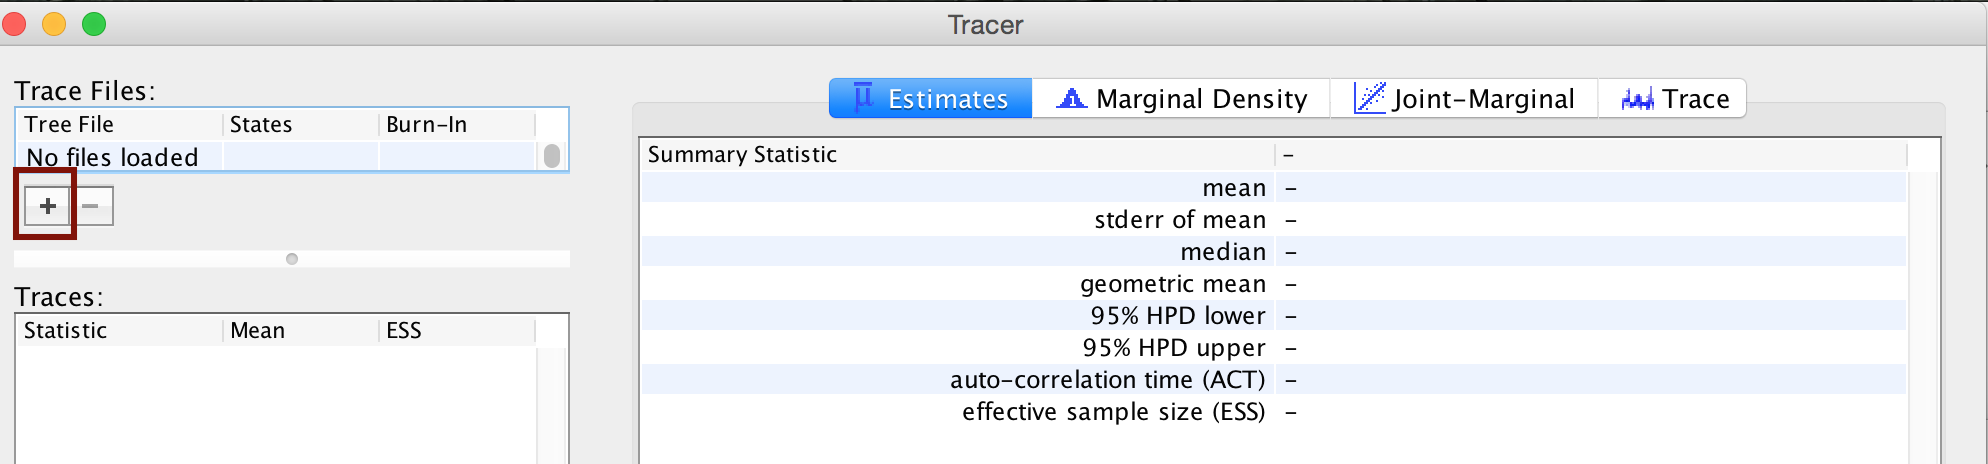
\includegraphics[width=\textwidth,angle=0]{\ResourcePath figures/tracer_load_file.png}
\caption{\small The {\tt Tracer} window. To add data, click on the ``+'' sign, highlighted in red above.}
\end{minipage}}
\label{fig:tracer}
\end{figure}


%Import the MCMC log file into Tracer.
\begin{framed}
Open {\tt Tracer} and import the \cl{bears.log} file in the \mi{File\textrightarrow Import New Trace File}.
Or click the \fbox{$+$} button on the left-hand side of the screen to add your log file (see Fig.\ \ref{fig:tracer}).
\end{framed}

\begin{figure}[h!]
\fbox{%
\begin{minipage}{\textwidth}\centering
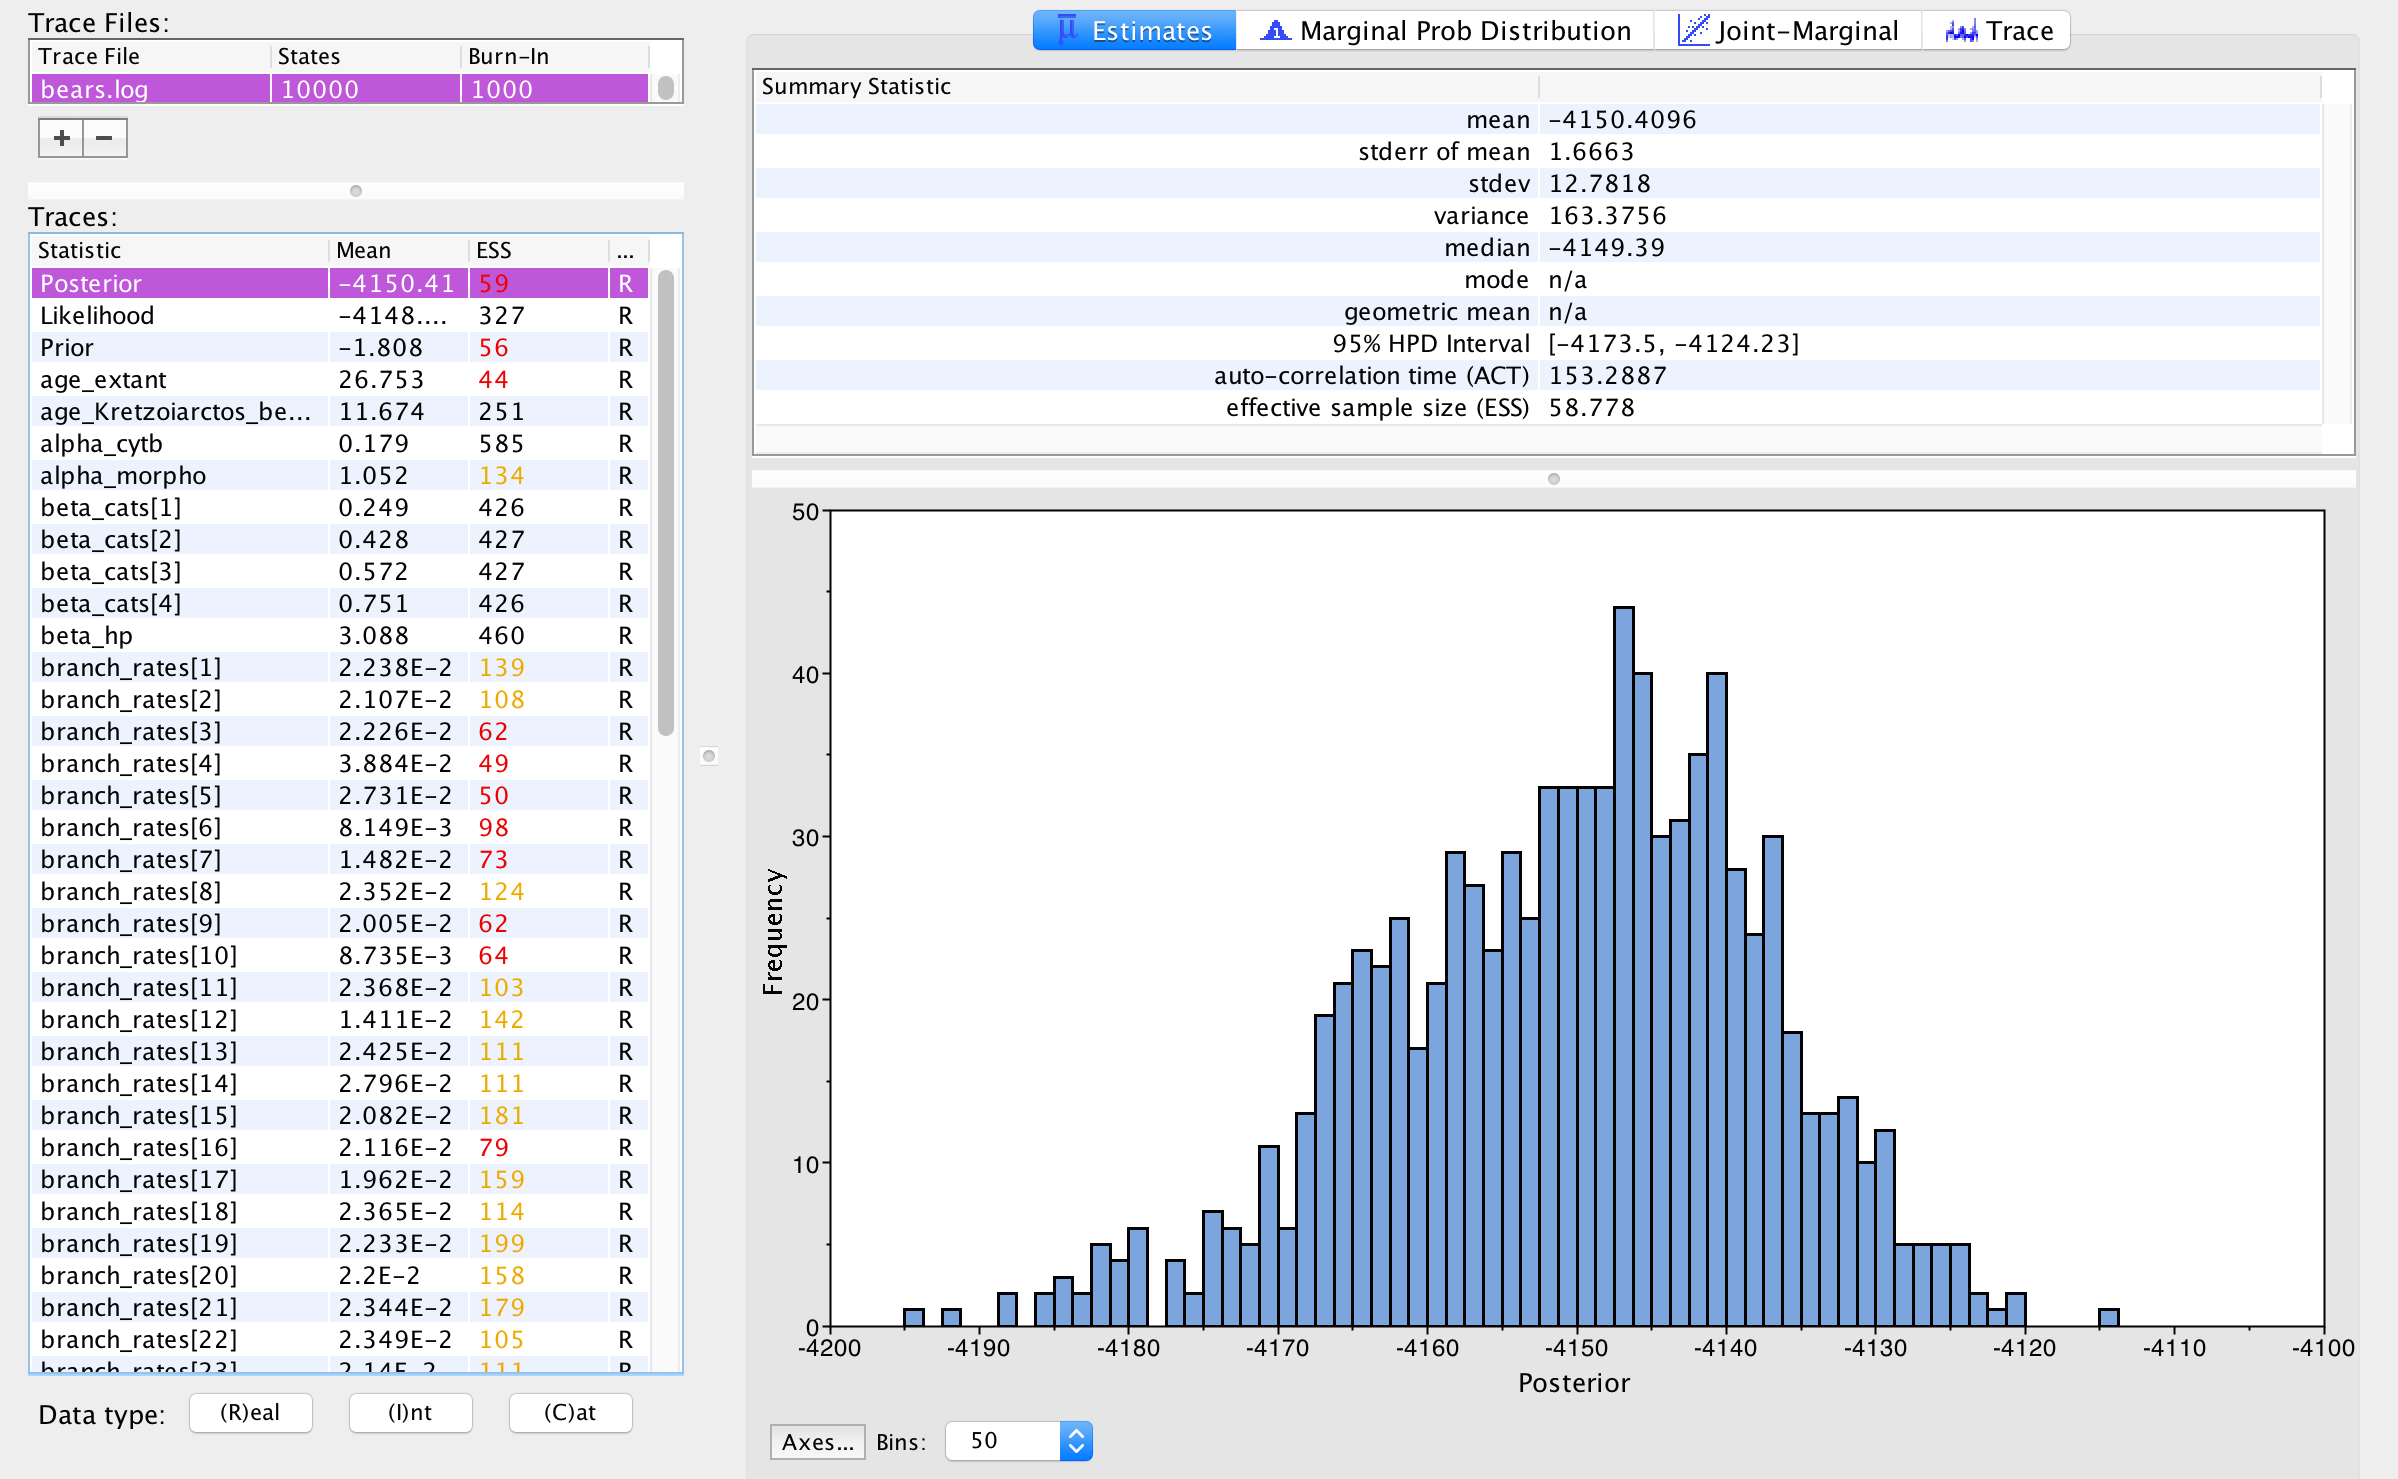
\includegraphics[width=\textwidth,angle=0]{\ResourcePath figures/tracer_fig_posterior_short.png}
\caption{\small The \mi{Estimates} window in {\tt Tracer} showing the histogram of the \mi{Posterior}.}
\end{minipage}}
\label{fig:tracer-post-ests}
\end{figure}


Immediately upon loading your file (see Fig.\ \ref{fig:tracer-post-ests}), 
you will see the list of \mi{Trace Files} on the left-hand side (you can load multiple files).
The bottom left section, called \mi{Traces}, provides a list of every parameter in the log file, along with the mean and the effective sample size (ESS) for the posterior sample of that parameter.
The ESS statistic provides a measure of the number of independent draws in our sample for a given parameter.
This quantity will typically be much smaller than the number of generations of the chain.
In {\tt Tracer}, poor to fair values for the ESS will be colored red and yellow.
You will likely see a lot of red and yellow numbers because the MCMC runs in this exercise are too short to effectively sample the posterior distributions of most parameters.
A much longer analysis is provided in the \cl{output} directory. 

The inspection window for your selected parameter is the \mi{Estimates} window, which shows a histogram and summary statistics of the values sampled by the Markov chain. 
Figure \ref{fig:tracer-post-ests} shows the marginal distribution of the \mi{Posterior} statistic for the \cl{bears.log} file in the \cl{output} directory.

%\begin{figure}[h!]
%\fbox{%
%\begin{minipage}{\textwidth}\centering
%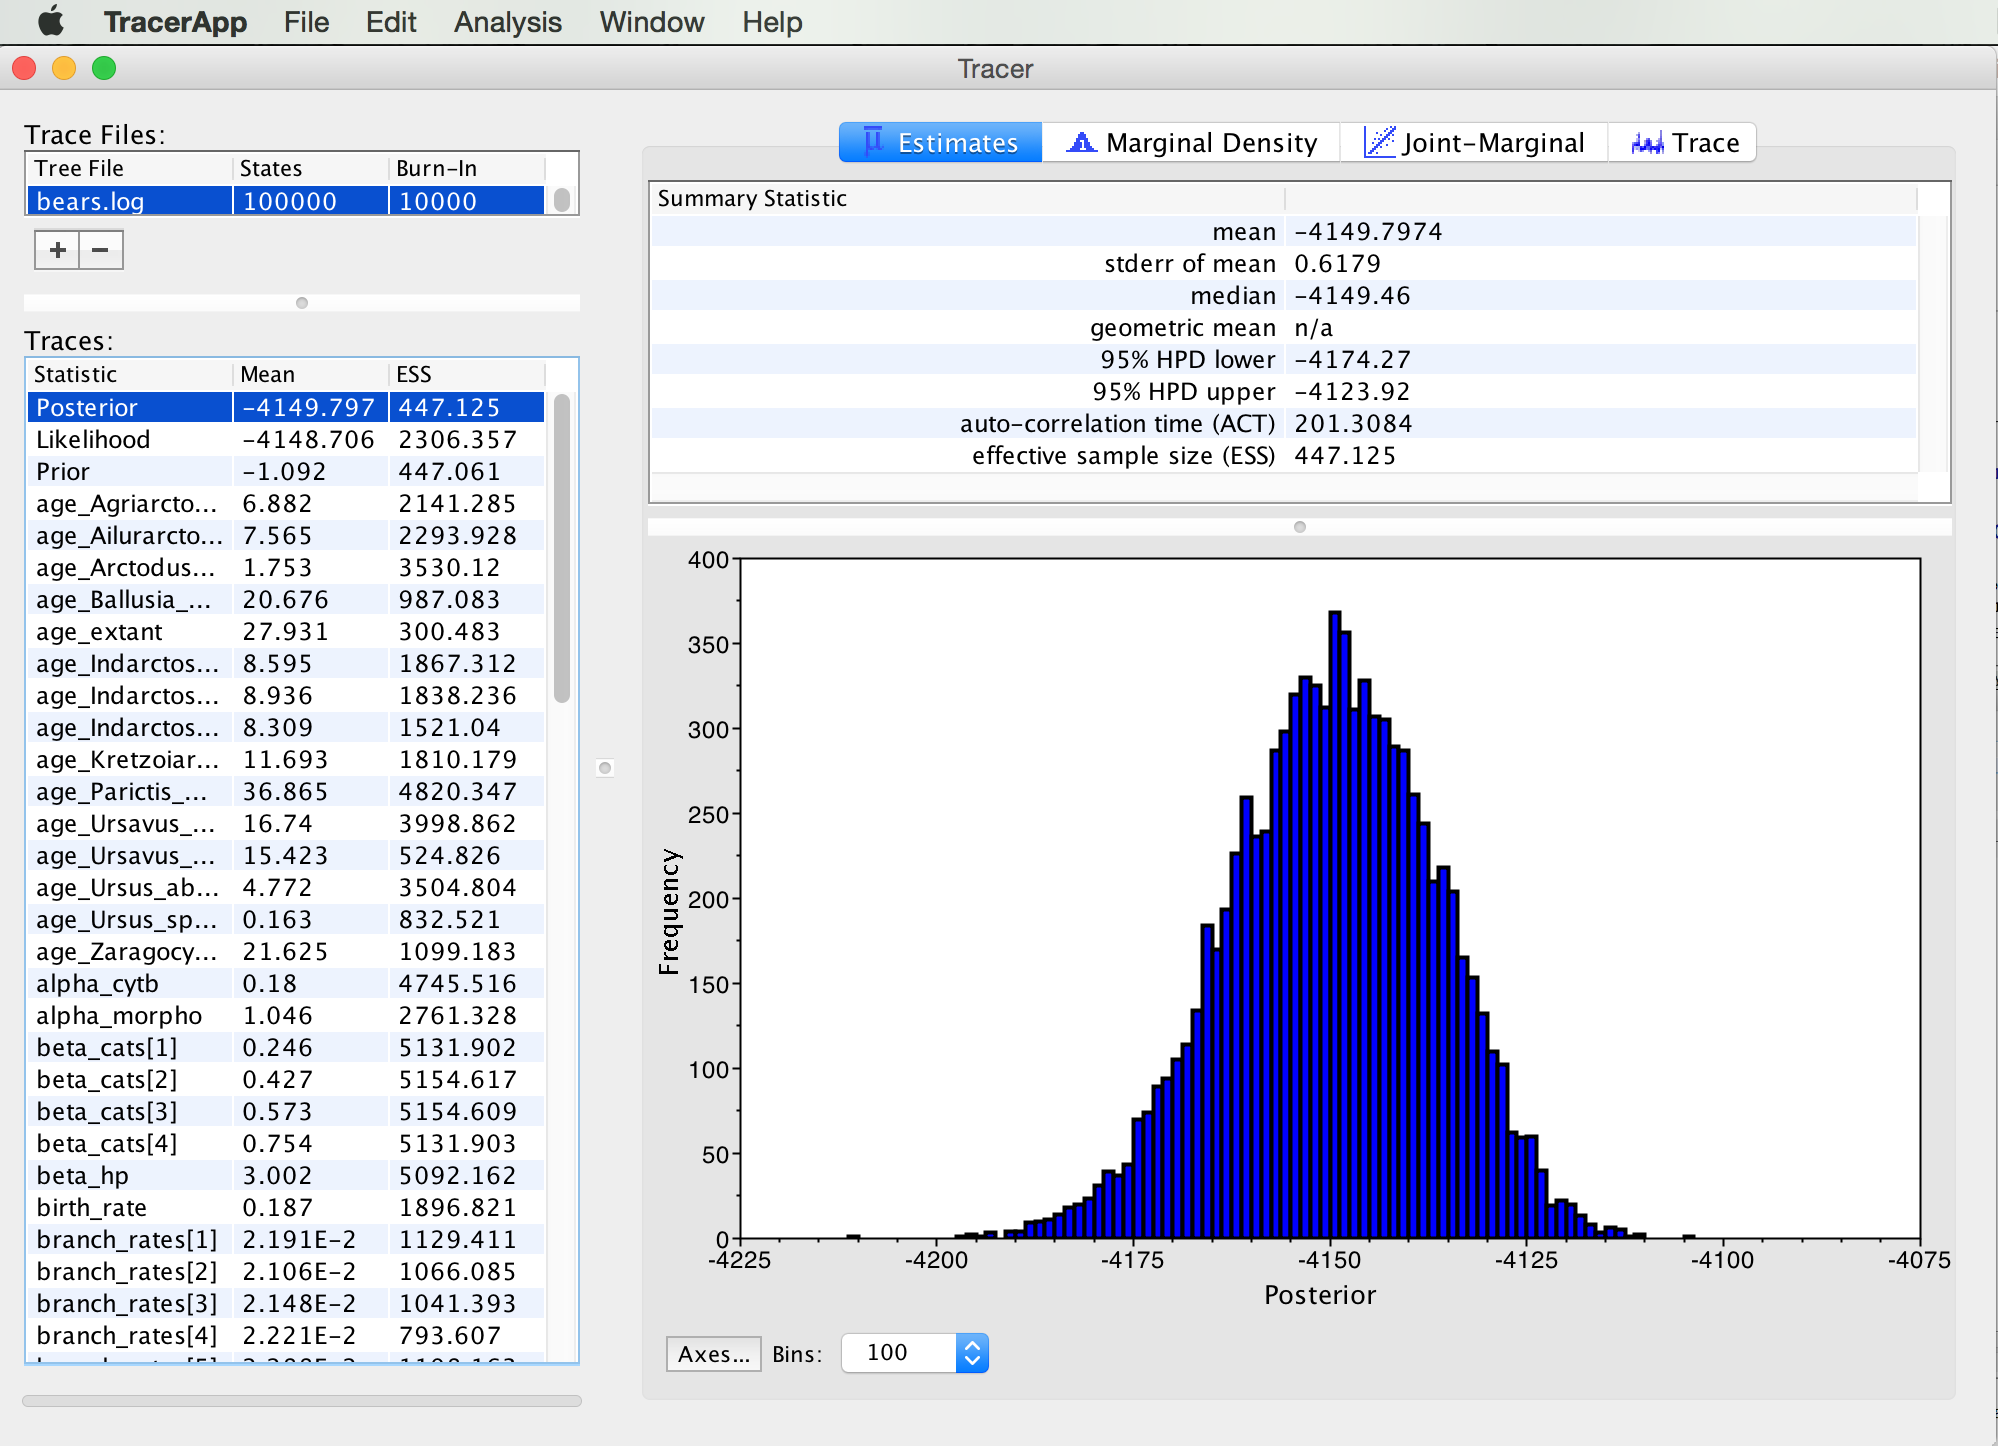
\includegraphics[width=\textwidth,angle=0]{\ResourcePath figures/samplewindow}
%\caption{\small The Estimates window. The left-hand window provides mean and ESS of the chain. The right-hand window visualizes the distribution of samples.}
%\end{minipage}}
%\label{fig:tracer}
%\end{figure}

\begin{framed}
Look through the various parameters and statistics in the list of \mi{Traces}. 

\QUEST Are there any parameters that have really low ESS? Why do you think that might be?
\end{framed}

Next, we can click over to the \mi{Trace} window.
This window shows us the samples for a given parameter at each iteration of the MCMC.
The left side of the chain has a shaded portion that has been excluded as ``burn-in''.
Samples taken near the beginning of chain are often discarded or ``burned'' because the MCMC may not immediately begin sampling from the target posterior distribution, particularly if the starting condition of the chain is far from the region of highest posterior density.
Figure \ref{fig:tracer-extinction-trace} shows the trace for the extinction rate.

\begin{figure}[h!]
\fbox{%
\begin{minipage}{\textwidth}\centering
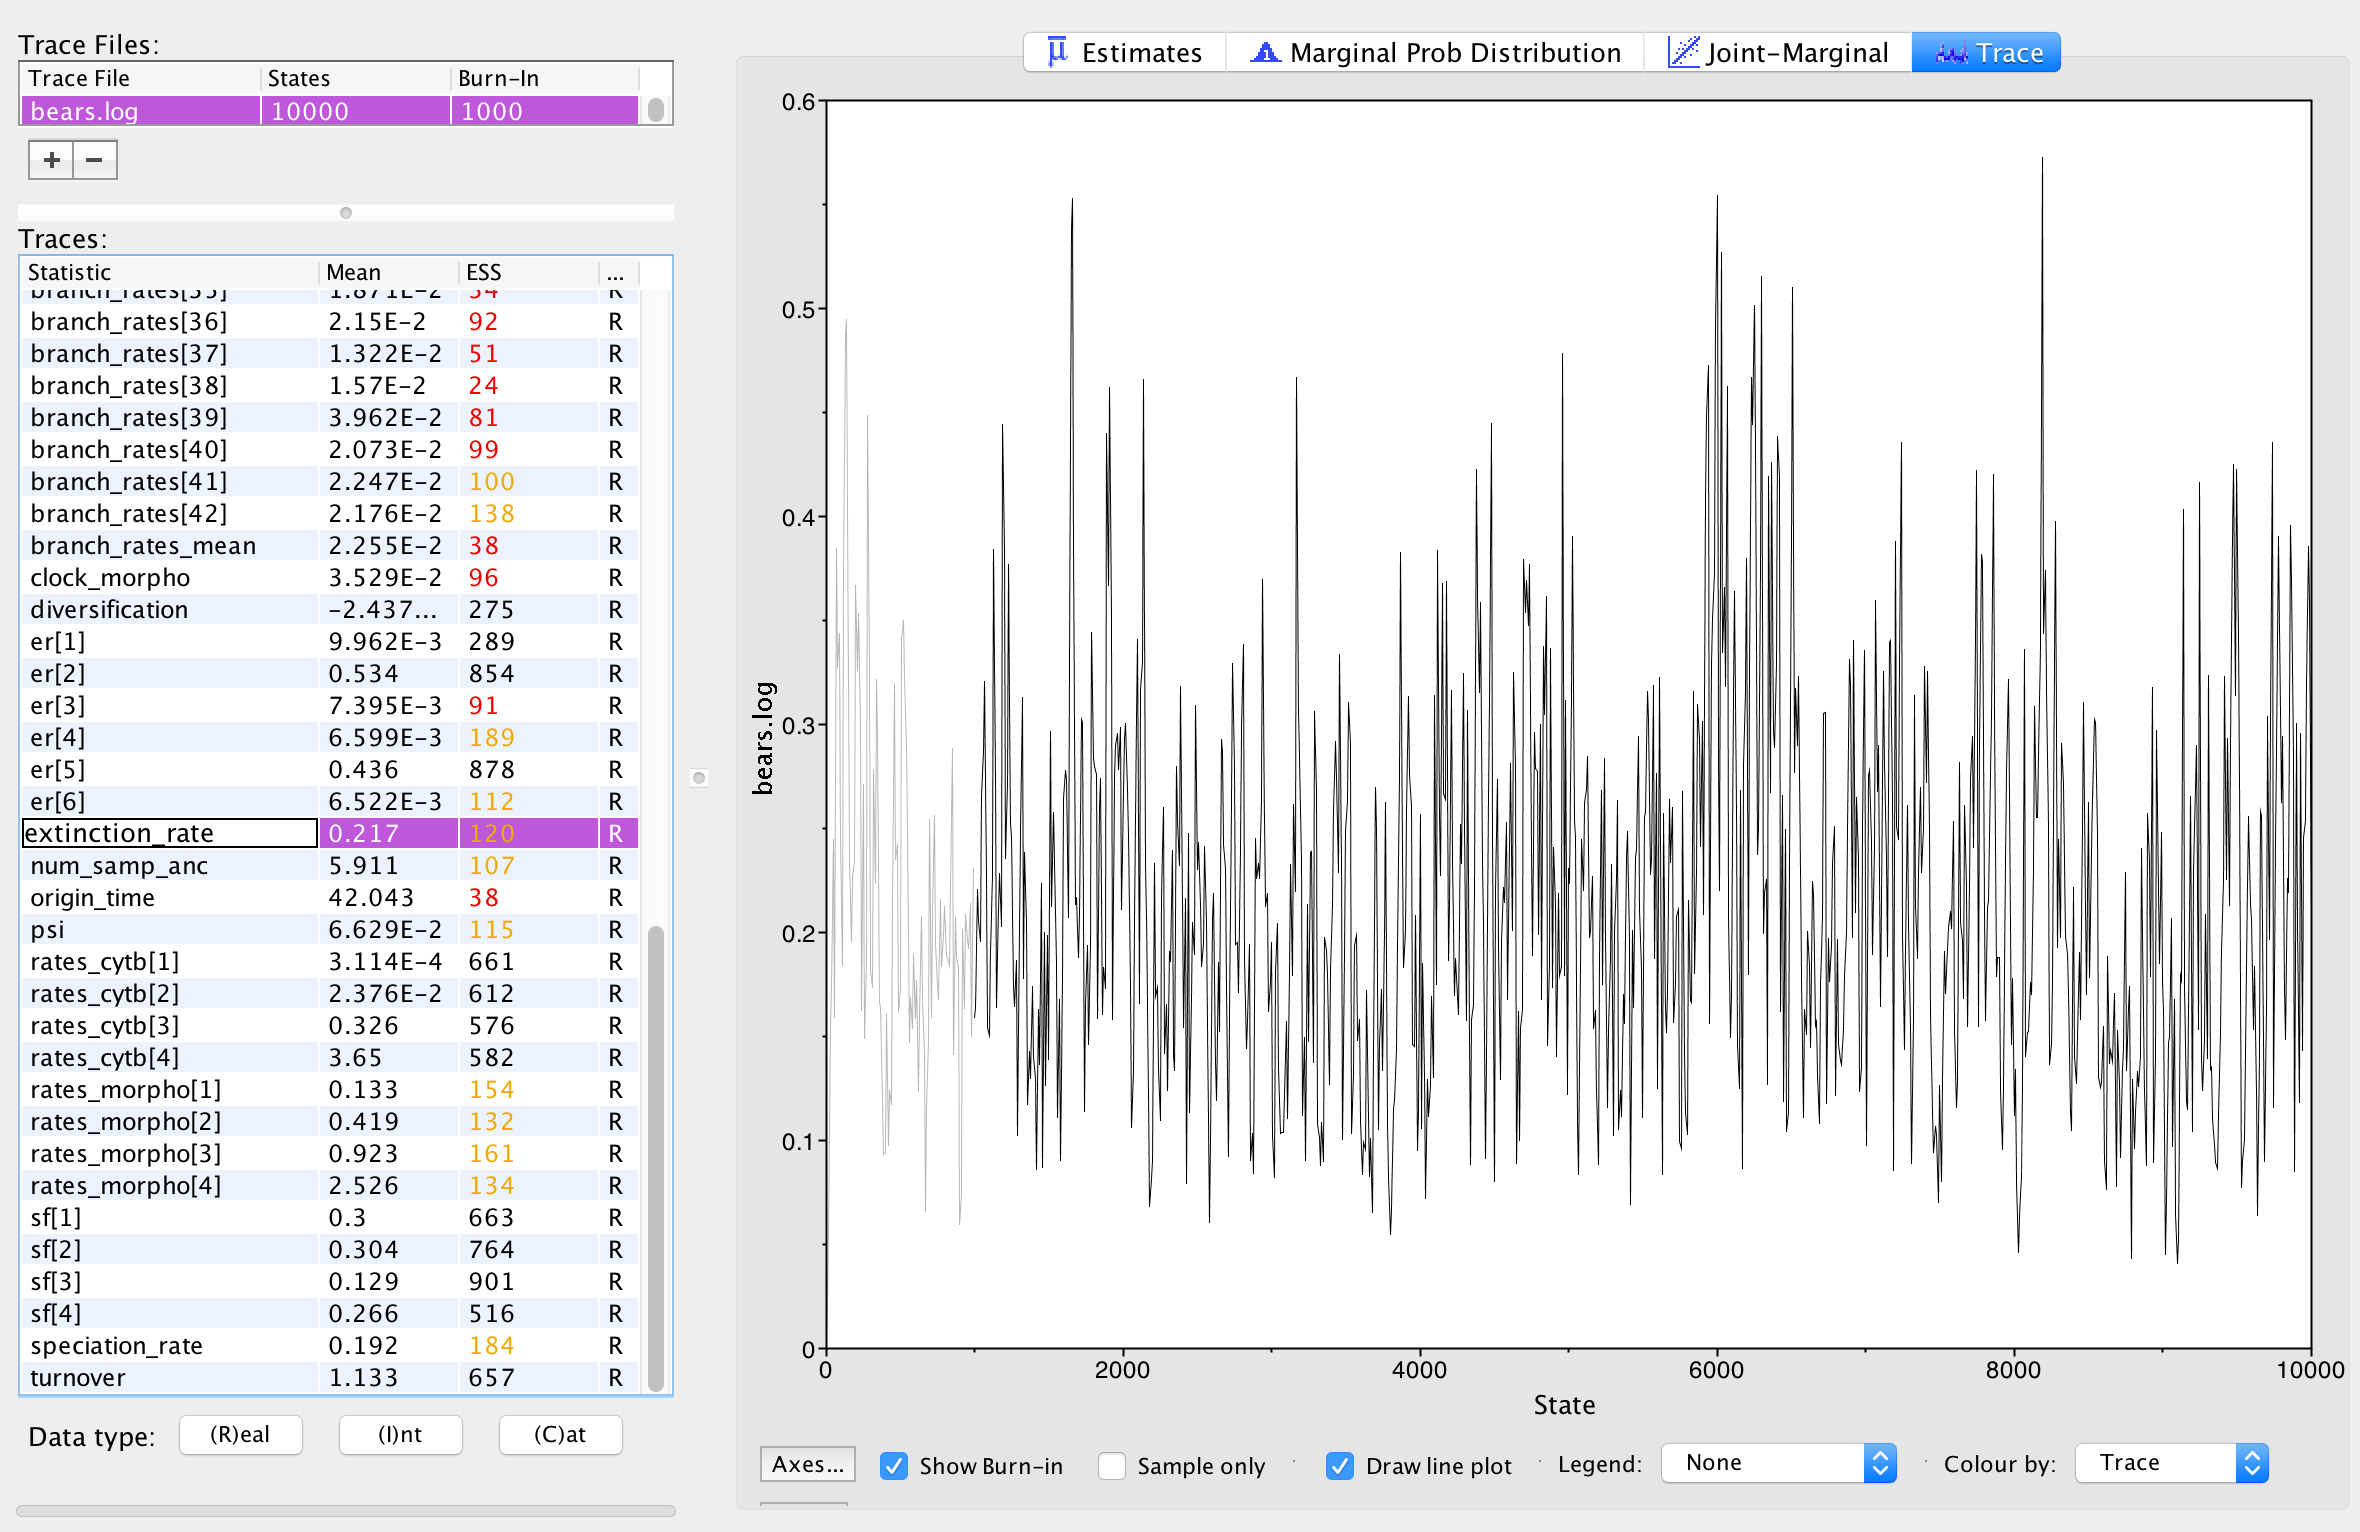
\includegraphics[width=\textwidth,angle=0]{\ResourcePath figures/tracer_extinction_rate_trace_short.png}
\caption{\small The \mi{Trace} window in {\tt Tracer}. This window shows a line plot of every sampled value for the extinction rate that was saved to file. The lighter shaded portion is the set of samples discarded as ``burn-in'' and are not used to compute the summary statistics found in the \mi{Estimates} window. }
\end{minipage}}
\label{fig:tracer-extinction-trace}
\end{figure}

The \mi{Trace} window allows us to evaluate how well our chain is sampling the target distribution.
For a fairly short analysis, the output in figure \ref{fig:tracer-extinction-trace} shows reasonable \textit{mixing}---there is no consistent pattern or trend in the samples, nor are there long intervals where the statistic does not change.
The presence of a trend or large leaps in a parameter value might indicate that your MCMC is not mixing well.
You can read more about MCMC tuning and improving mixing in the tutorials \href{https://github.com/revbayes/revbayes_tutorial/raw/master/tutorial_TeX/RB_MCMC_Intro_Tutorial/RB_MCMC_Intro_Tutorial.pdf}{\mi{Intro to MCMC}} and \href{https://github.com/revbayes/revbayes_tutorial/raw/master/tutorial_TeX/RB_MCMC_Tutorial/RB_MCMC_Tutorial.pdf}{\mi{MCMC Algorithms}}.

\begin{framed}
Look through the traces for your parameters. 

\QUEST Are there any parameters in your log files that show trends or large leaps? What steps might you take to solve these issues?
\end{framed}

In {\tt Tracer} you can view the marginal probability distributions of your parameters in the \mi{Marginal Prob Distribution} window. 
Using this tool, you can compare the distributions of several different parameters (by selecting them both).

\begin{framed}
Go to the \cl{diversification} parameter in the \mi{Marginal Prob Distribution} window.

\QUEST What is the mean value estimated for the net diversification rate ($d$)? What does the marginal distribution tell you about the net diversification? (Hint: $d = \lambda - \mu$)
\end{framed}

While specifying the model, remember that we created several deterministic nodes that represent parameters that we would like to estimate, including the net diversification rate. 
{\tt Tracer} allows us to view the summaries of these parameters since they appear in our log files.

\begin{framed}
Go to the \cl{age\_extant} parameter in the \mi{Estimates} window.

\QUEST What is the mean and 95\% highest posterior density of the age of the MRCA for all living bears? 
\end{framed}


Since you have evaluated several of the parameters by viewing the trace files and the ESS values, you may be aware that the MCMC analysis you conducted for this tutorial did not sufficiently sample the joint posterior distribution of phylogenetic parameters.
More explicitly, \textit{your run has not converged}.
It is not advisable to base your conclusions on such a run and it will be critical to perform multiple, independent runs for many more MCMC cycles. 
For further discussion of recommended MCMC practices in \RevBayes, please see the \href{https://github.com/revbayes/revbayes_tutorial/raw/master/tutorial_TeX/RB_MCMC_Intro_Tutorial/RB_MCMC_Intro_Tutorial.pdf}{\mi{Intro to MCMC}} and \href{https://github.com/revbayes/revbayes_tutorial/raw/master/tutorial_TeX/RB_MCMC_Tutorial/RB_MCMC_Tutorial.pdf}{\mi{MCMC Algorithms}} tutorials.

\medskip
\subsubsection{Summarize Tree}\label{subsub:Exercise-SummarizeTree}

%TODO this they can do interactively in rb

In addition to evaluating the performance and sampling of an MCMC run using numerical parameters, it is also important to inspect the sampled topology and tree parameters. 
This is a difficult endeavor, however. 
One tool for evaluating convergence and mixing of the tree samples is \href{https://github.com/danlwarren/RWTY}{\tt RWTY} \citep{Warren2016}. 
In this tutorial, we will only summarize the sampled trees, but we encourage you to consider approaches for assessing the performance of the MCMC with respect to the tree topology.

Ultimately, we are interested in summarizing the sampled trees and branch times, given that our MCMC has sampled all of the important parameters in proportion to their posterior probabilities. 
\RevBayes includes some functions for summarizing the tree topology and other tree parameters.


{\begin{framed}
We will complete this part of the tutorial using \RevBayes interactively.
Begin by running the \RevBayes executable. 
You should do this from within the \cl{RB\_TotalEvidenceDating\_FBD\_Tutorial} directory.

In Unix systems, type the following in your terminal (if the \RevBayes binary is in your path):

\colorbox{black}{\strut\hspace{1mm}\textcolor[rgb]{0,1,1}{\cl{rb}}\hspace{0.925\textwidth}}
\end{framed}}


Read in the MCMC sample of trees from file.
{\tt \begin{snugshade*}
\begin{lstlisting}
trace = readTreeTrace("output/bears.trees")
\end{lstlisting}
\end{snugshade*}}

The first thing we need to do is remove taxa for which we did not have any molecular or morphological data.
The phylogenetic placement of these taxa is based only on their occurrence times and any clade constraints we applied (section \ref{subsub:Exercise-FBD-Constraints}). 
Because no data are available to resolve their relationships to other lineages, we will treat their placement as \href{https://en.wikipedia.org/wiki/Nuisance_parameter}{\textit{nuisance parameters}} and remove them from the summary tree.

We must read our complete taxon list into \RevBayes so that we can easily access the taxon names of the lineages we'd like to prune.
{\tt \begin{snugshade*}
\begin{lstlisting}
taxa <- readTaxonData("data/bears_taxa.tsv")
\end{lstlisting}
\end{snugshade*}}

We will 
%use the \cl{fnPruneTree()} function to 
remove two fossil taxa, \textit{Parictis montanus} and \textit{Ursus abstrusus}, from every tree in the trace file before summarizing the samples.
These two species have the indices \cl{17} and \cl{20} in our list of taxa. 
You can view the list by typing its variable name \cl{taxa}:
{\tt \begin{snugshade*}
\begin{lstlisting}
taxa 
|*  [ Ailuropoda_melanoleuca, Helarctos_malayanus, Melursus_ursinus, Tremarctos_ornatus,
|*  Ursus_americanus, Ursus_arctos, Ursus_maritimus, Ursus_thibetanus, Agriarctos_spp,
|*  Ailurarctos_lufengensis, Arctodus_simus, Ballusia_elmensis, Indarctos_arctoides,
|*  Indarctos_punjabiensis, Indarctos_vireti, Kretzoiarctos_beatrix, Parictis_montanus,
|*  Ursavus_brevirhinus, Ursavus_primaevus, Ursus_abstrusus, Ursus_spelaeus, Zaragocyon_daamsi]
\end{lstlisting}
\end{snugshade*}}

Use the \cl{fnPruneTree()} function to prune taxon \cl{17} and taxon \cl{20} from each tree using a \cl{for} loop.
We'll store each new tree in the vector called \cl{trees}.

{\tt \begin{snugshade*}
\begin{lstlisting}
for(i in 1:trace.size())
{
    trees[i] = fnPruneTree(trace.getTree(i), pruneTaxa=v(taxa[17],taxa[20]))
}
\end{lstlisting}
\end{snugshade*}}

Then we create a second tree trace containing the pruned trees using the \cl{treeTrace} function.

{\tt \begin{snugshade*}
\begin{lstlisting}
trace_pruned = treeTrace(trees)
\end{lstlisting}
\end{snugshade*}}

If you use the size function of the \cl{trace\_pruned} variable by typing the command \colorbox{shadecolor}{\cl{trace\_pruned.size()}}, you will see that our MCMC sampled 1001 trees. 
By default, a burn-in of 25\% is used when creating the tree trace (250 trees in our case). You can specify a different burn-in fraction, say 50\%, by typing the command \colorbox{shadecolor}{\cl{trace\_pruned.setBurnin(0.5)}}.

Now we will use the \cl{mccTree()} function to return a maximum clade credibility (MCC) tree.
The MCC tree is the tree with the maximum product of the posterior clade probabilities.
When considering trees with sampled ancestors, we refer to the maximum sampled ancestor clade credibility (MSACC) tree \citep{Gavryushkina2016}.
We also use the option \cl{conditionalAges=false} to indicate that the node ages of the output tree should not be summarized conditional on the MCC topology.
{\tt \begin{snugshade*}
\begin{lstlisting}
mccTree(trace_pruned, file="output/bears.mcc.tre", conditionalAges=false )
\end{lstlisting}
\end{snugshade*}}


When there are sampled ancestors present in the tree, visualizing the tree can be fairly difficult in traditional tree viewers.
We will make use of a browser-based tree viewer called \href{http://tgvaughan.github.io/icytree/}{\tt IcyTree}, created by \href{https://github.com/tgvaughan}{Tim Vaughan}.
{\tt IcyTree} has many unique options for visualizing phylogenetic trees and can produce publication-quality vector image files (\IE SVG). 
Additionally, it correctly represents sampled ancestors on the tree as nodes, each with only one descendant (Fig.\ \ref{fig:IcyTreeSumm}). 
\begin{figure}[h!]
\fbox{%
\begin{minipage}{\textwidth}\centering
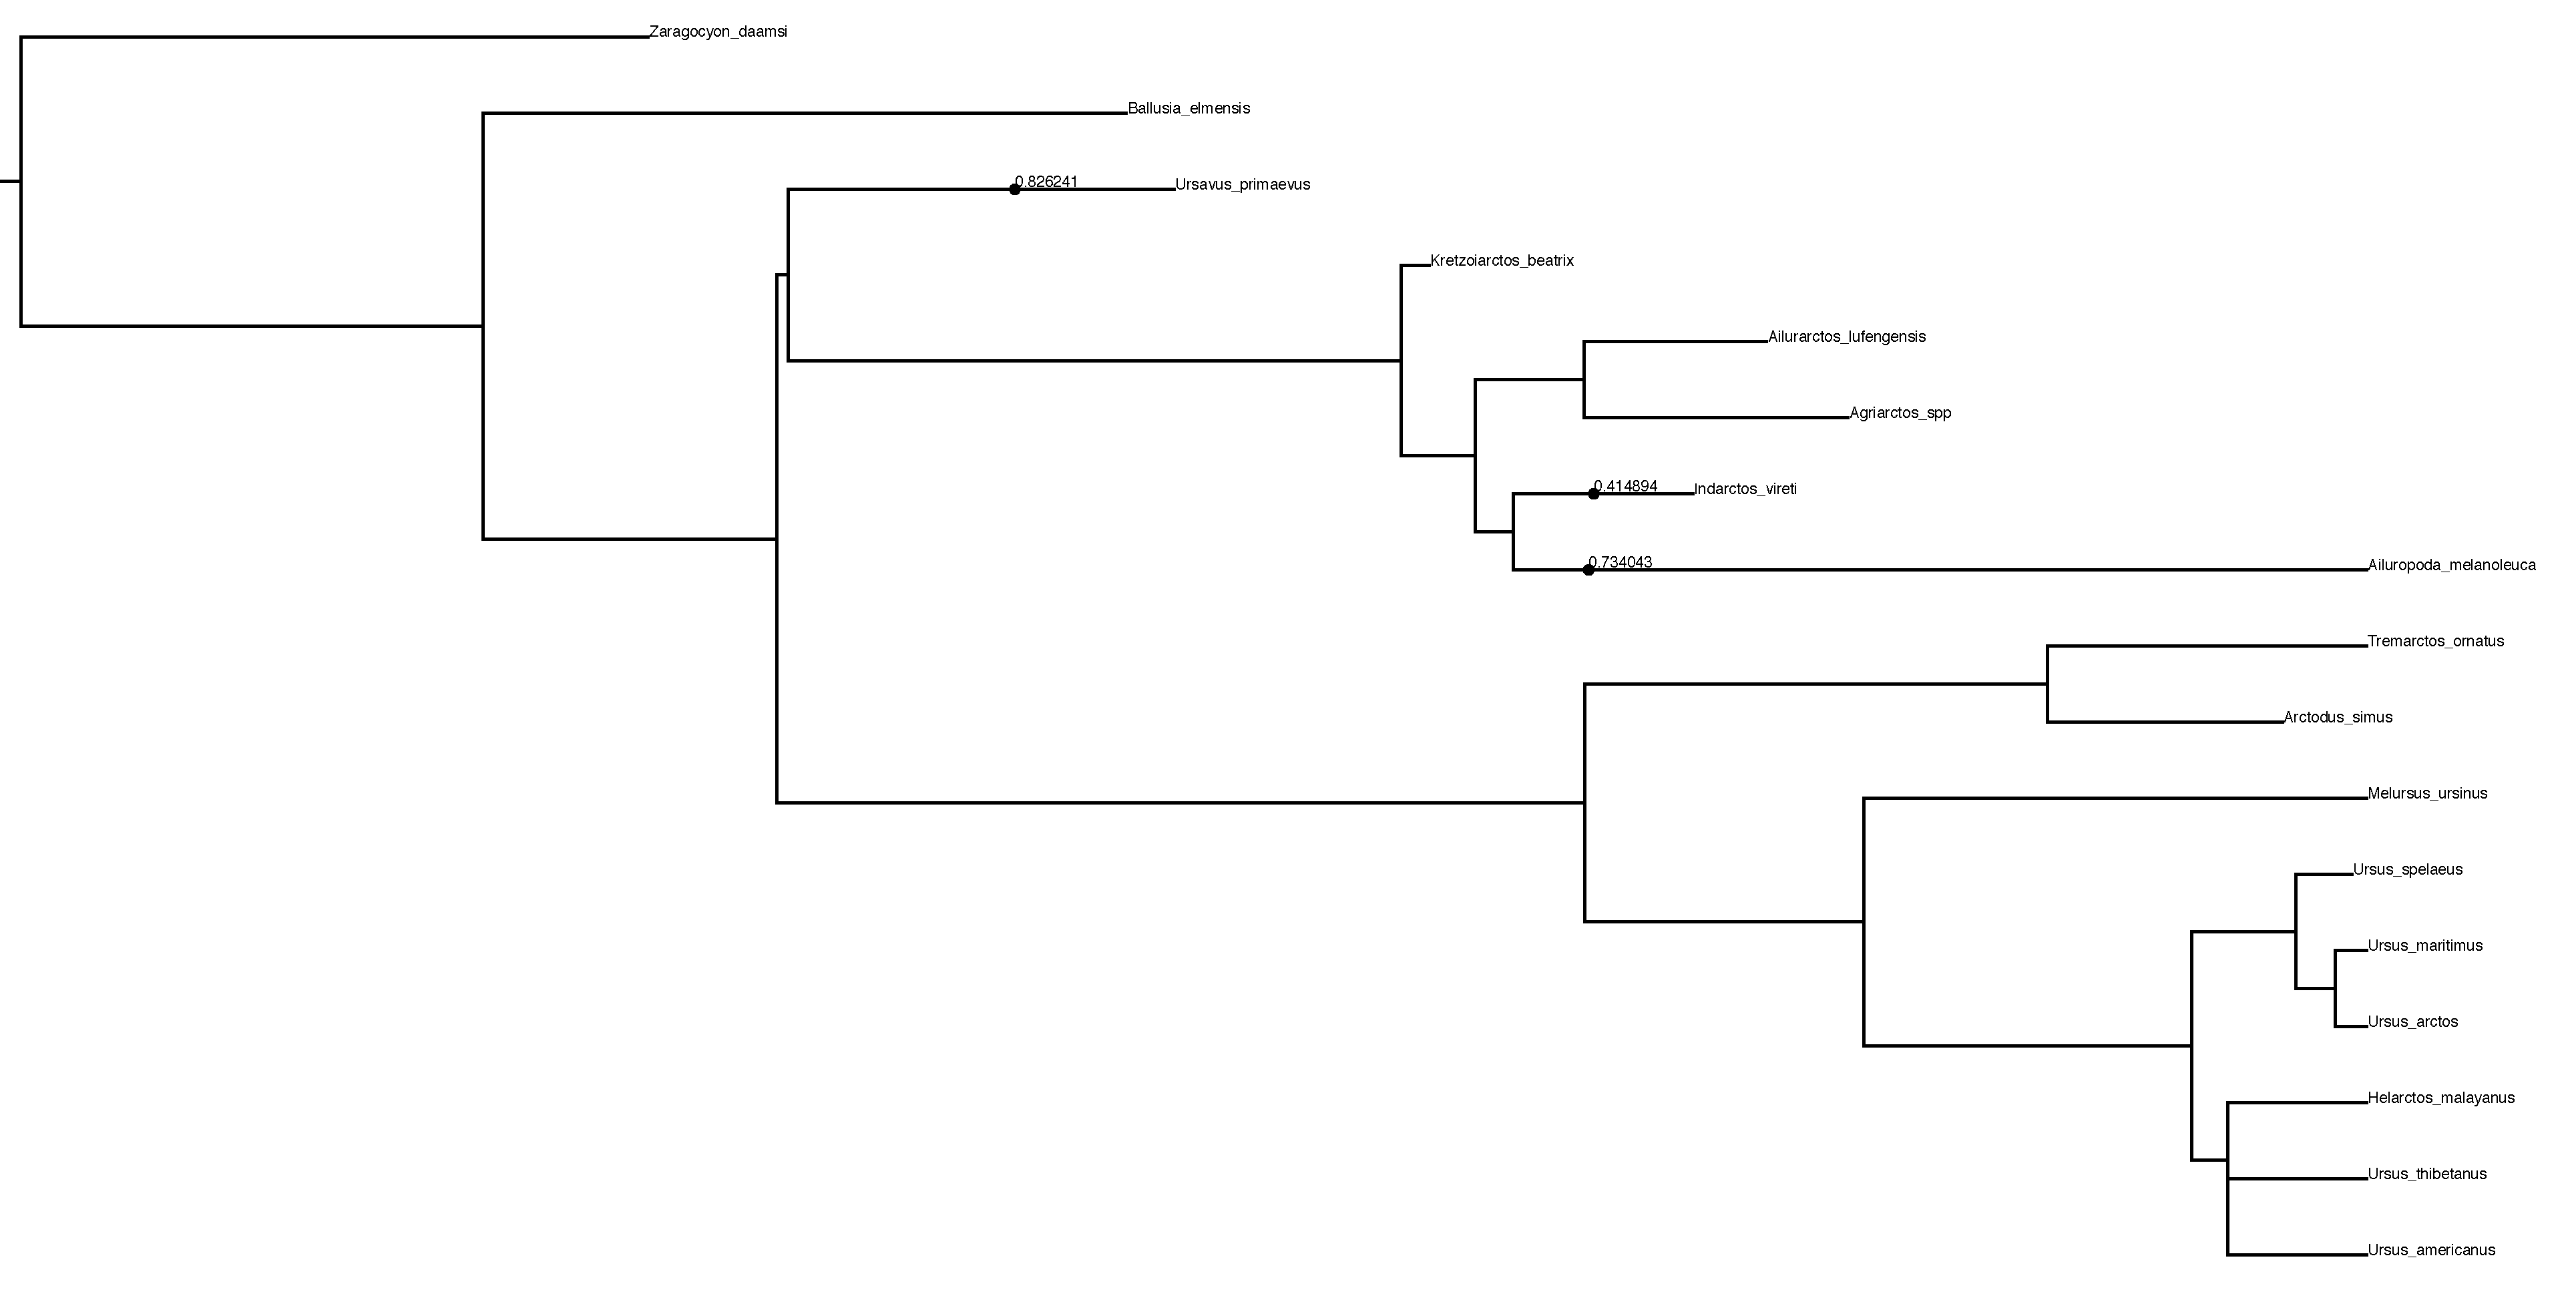
\includegraphics[width=\textwidth,angle=0]{\ResourcePath figures/summary_tree.pdf}
\caption{\small Maximum sampled ancestor clade credibility (MSACC) tree of bear species used in this tutorial. Numbers above fossil nodes indicate the posterior probability of being a sampled ancestor.}
\end{minipage}}
\label{fig:IcyTreeSumm}
\end{figure}

{\begin{framed}
Navigate to \url{http://tgvaughan.github.io/icytree} and open the file \cl{output/bears.mcc.tre} in {\tt IcyTree}.

\QUEST Try to replicate the tree in Fig.\ \ref{fig:IcyTreeSumm}. (Hint: \mi{Style\textrightarrow Mark Singletons})
Why might a node with a sampled ancestor be referred to as a singleton? 

\QUEST How can you see the names of the fossils that are putative sampled ancestors?

\QUEST Try mousing over different branches (see Fig\ \ref{fig:IcyTreeScreenshort}).
What are the fields telling you?
%Is the age of the \textit{Kretzoiarctos beatrix} fossil the same as what was shown in {\tt Tracer}? 

\QUEST What is the posterior probability that \textit{Zaragocyon daamsi} is a sampled ancestor?

Another newly available web-based tree viewer is \href{http://phylogeny.io/}{Phylogeny.IO} \citep{Jovanovic2016}. 
Try this site for a different way to view the tree.
\end{framed}}



%TODO more here, create final tree image


\begin{figure}[h!]
\fbox{%
\begin{minipage}{\textwidth}\centering
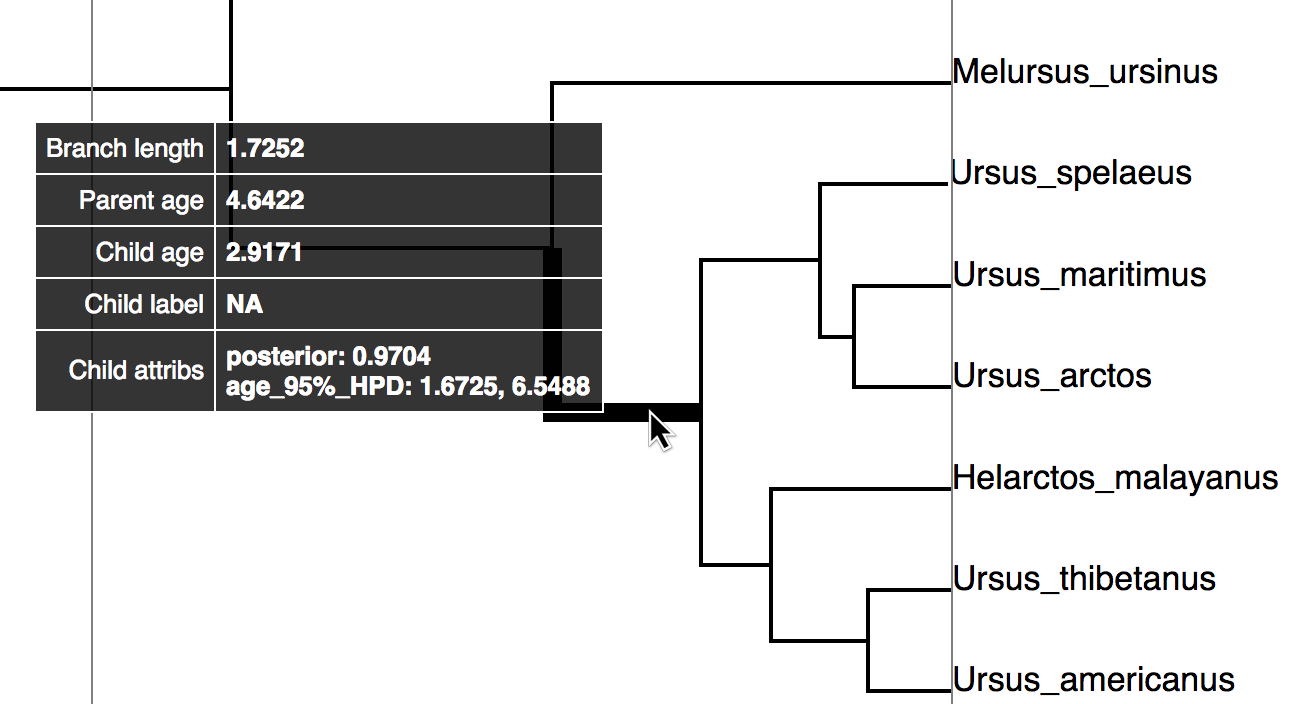
\includegraphics[scale=0.45, angle=0]{\ResourcePath figures/branch_highlight.png}
\caption{\small Screenshot of highlighting a branch in {\tt IcyTree} showing child node attributes, including the clade posterior probability and the 95\% highest posterior density (HPD) age interval.}
\end{minipage}}
\label{fig:IcyTreeScreenshort}
\end{figure}



%TODO IcyTree

\bibliographystyle{sysbio}
\bibliography{\GlobalResourcePath refs}

